\documentclass[a4paper,10pt,twoside,frenchb]{report}
\usepackage{babel}
\usepackage[T1]{fontenc}
\usepackage[utf8]{inputenc}
\usepackage{natbib}
\usepackage{fancyhdr}
\usepackage{indentfirst}
\usepackage{vmargin}
\usepackage{verbatim}
\usepackage{xspace}
\usepackage{graphicx}
\usepackage[sf,bf]{titlesec}
\usepackage{listings}
\usepackage{booktabs}
\usepackage{array}
\usepackage{dcolumn}
\usepackage{float}
\usepackage{color}
\usepackage{varioref}
\usepackage{amsmath}
\usepackage{lmodern}
\usepackage[normalem]{ulem}
\usepackage[autolanguage]{numprint}
\usepackage[colorlinks=true,urlcolor=blue,citecolor=magenta]{hyperref}

\frenchbsetup{FrenchFootnotes=true,ThinSpaceInFrenchNumbers=true}

\bibliographystyle{plainnat-fr}
\renewcommand{\cite}{\citep}

%% Nouveau type de colonne, centré sur le . en séparateur décimal,
%% remplacé par une virgule en sortie. Le nombre de chiffres après la
%% virgule est passé en argument. exemple d'usage : d{2}
\newcolumntype{d}[1]{D{.}{,}{#1}}

\newcommand{\chid}{$\chi^2$\xspace}
\newcommand{\chidpdf}{\texorpdfstring{$\chi^2$\xspace}{X\texttwosuperior\xspace}}
\newcommand{\margpar}[1]{\marginpar{\raggedright \small \textit{#1}}}

%\newcommand{\version}{3.2\xspace}

%\setmarginsrb{left}{top}{right}{bottom}{headheight}{headsep}{footheight}{footsep}
%\setmarginsrb{2.5cm}{1.5cm}{2.5cm}{2cm}{1cm}{1cm}{1cm}{1cm}
%\setcounter{tocdepth}{2}
%\definecolor{grisclair}{gray}{0.97}

\title{Tout ce que vous n'avez jamais voulu savoir sur le \chid sans
  jamais avoir eu envie de le demander}
\author{Julien Barnier\\ Centre Max Weber\\
  CNRS -- UMR 5283\\ \href{mailto:julien.barnier@ens-lyon.fr}{\texttt{julien.barnier@ens-lyon.fr}}}
\date{\today{}}
%\abstract{}

\begin{document}

\renewcommand\chaptername{Partie}

\maketitle
\thispagestyle{empty}

%\newpage
\pagestyle{fancy}
\renewcommand{\chaptermark}[1]{\markboth{#1}{}}
\renewcommand{\sectionmark}[1]{\markright{\thesection.\ #1}}
\fancyhead{}
\fancyhead[RO,LE]{\thepage}
\fancyhead[RE]{\nouppercase{\leftmark}}
\fancyhead[LO]{\nouppercase{\rightmark}}
\fancyfoot{}
%\lhead[]{\leftmark}
%\rhead[]{\rightmark}
%\cfoot{\thepage}

\tableofcontents

%\listoffigures
%\newpage

\sloppy

\setlength{\parskip}{1.5ex}


\chapter{Introduction}

\section{À propos de ce document}

Ce document a pour ambition d'essayer de présenter les principes du
test statistique dit \og test du \chid \fg{}, autant que possible de
manière pas trop rébarbative.

On insistera très peu sur le mode de calcul effectif (tous les
logiciels de statistiques actuels s'en chargent bien mieux que nous)
et beaucoup plus sur les concepts sur lesquels le test repose.

La version de référence de ce document ainsi que le code source
\LaTeX{} sont disponibles à l'adresse~:

\url{https://github.com/juba/archive_doc_khi2}

Tous les fichiers relatifs à ce document sont diffusés sous licence
\href{http://creativecommons.org/licenses/by/2.0/fr/}{\textit{Creative commons}}.

\textbf{Contributions~: } nos remerciements à Denis Duplan pour sa
remarque sur l'utilisation des carrés des écarts, et à Julien Biaudet
pour avoir pris le temps de nous signaler plusieurs coquilles.

\section{Mode d'emploi}

À l'image de son titre, ce document est long. Très long. Trop long.

La lecture intégrale de ce document pourrait avoir des conséquences en
termes d'équilibre psychique et d'exacerbation de sentiments
agressifs à l'égard de son prochain que nous ne saurions évaluer de
manière parfaitement rigoureuse. Le principe de précaution nous dicte
donc de prévoir des modes de lecture alternatifs.

Voici donc un plan rapide de ce qui suit afin que ceux qui le
souhaitent n'aient pas à supporter la lecture de l'ensemble~:

\begin{itemize}
\item la partie~\ref{sec-indep} présente l'hypothèse d'indépendance,
  qui est au c\oe{}ur du test du \chid. La partie~\ref{sec-indepcalc}
  présente la manière dont cette hypothèse d'indépendance se traduit
  par le calcul d'un tableau d'effectifs théoriques~;
\item la partie~\ref{sec-calcchid} présente les différentes étapes de
  calcul du \chid d'un tableau et les résultats qu'on peut en tirer~;
\item la partie~\ref{sec-interp} se penche sur l'interprétation qui
  peut être faite des résultats du \chid, et notamment sur les facteurs
  qui influencent la valeur du test~;
\item la partie~\ref{sec-limites} aborde les limites liées au test et
  qu'il faut prendre en compte dans l'interprétation~;
\item la partie~\ref{sec-raffin} indique des subtilités ou des
  compléments au test. Elle peut être joyeusement ignorée en cas de
  première lecture.
\end{itemize}

Enfin, la partie~\ref{sec-aidem} se veut un récapitulatif des
différents points importants à retenir. Chacun d'entre eux est
accompagné du numéro de la page correspondant si on souhaite un peu
plus de détail. Cette partie peut être utilisée comme \og porte
d'entrée \fg{} pour le reste du document si on ne souhaite pas une
lecture linéaire intégrale.


\section{Le test du quoi~?}

Première interrogation~: comment ça se prononce~?

Le $\chi$ n'est pas un X mais bien une lettre grecque dont le petit
nom est \textit{khi}, lequel se prononce \textit{\og qui \fg{}}. Et le
$^2$, qui pourrait se prononcer \textit{\og au carré \fg{}}, se prononce
plutôt tout simplement \textit{\og deux \fg{}}.

Moralité, si vous souhaitez briller dans un congrès international de
statistiques, dites \textit{\og test du qui-deux \fg{}} plutôt que
\textit{\og test du x-au-carré \fg{}}\footnote{Quoi que l'expression
  \textit{\og qui-carré \fg{}} semble également tout à fait acceptable,
  d'autant que la version anglaise est \textit{\og chi squared \fg{}}.}.

\section{Et sinon, ça sert à quoi~?}

En une phrase, le test du \chid permet de déterminer la probabilité
que les lignes et les colonnes d'un tableau croisé sont
indépendantes\footnote{Note pour les puristes~: nous n'abordons dans
  ce document que le test du \chid de contingence, c'est-à-dire celui
  qui teste l'indépendance des lignes et des colonnes d'un tableau
  croisé. On ne parlera pas des autres applications de la statistique
  du \chid, notamment pour tester l'adéquation à une loi ou à une
  répartition donnée.}.

Dit autrement, il permet d'évaluer si la répartition des effectifs
dans une table de contingence est significativement différente de
celle de la table calculée sous l'hypothèse d'indépendance des deux
variables croisées.

Comme tout cela est absolument incompréhensible, nous allons commencer
par définir les concepts de base, et en premier lieu le terme
d'\textit{indépendance}.



\chapter{L'hypothèse d'indépendance}
\label{sec-indep}

\section{Petits rappels}
\label{ssec-tabcrois}

Une variable qualitative est une variable qui mesure une donnée
pouvant être découpée en un nombre restreint de modalités, par
exemple~:

\begin{itemize}
\item le genre de l'enquêté~: homme, femme~;
\item la couleur de son arrosoir~: vert, rouge, bleu, noir\ldots~;
\item son âge en classes de cinq ans~: 21-25 ans, 26-30 ans, 31-35
  ans\ldots~;
\item le dernier livre qu'il a lu~: \textit{Tractatus logico-philosophicus},
  \textit{Oui-oui et la voiture jaune}\ldots\\
\end{itemize}

Une table de contingence, ou tableau croisé, est un tableau qui
indique les effectifs du croisement entre deux variables qualitatives.

Un petit exemple, croisant l'âge et le dernier livre lu par la
personne interrogée~:

\begin{center}
  \begin{tabular}[!h]{>{\itshape}lrrr}
    \toprule
    & 0 à 10 ans &  11 à 70 ans & 71 ans et plus\\
    \midrule
    Tractatus Logico-philosophicus &   1 &   15 & 2 \\
    Oui-oui et la voiture jaune  &    \nombre{854} &   2 & \nombre{621} \\
    \bottomrule
  \end{tabular}
\end{center}

Sur ce genre de tableau, on peut regarder quelle est la répartition
âges des lecteurs de chaque ouvrage. Pour cela on calcule les
\textit{pourcentages en ligne}, c'est à dire qu'on divise les
effectifs de chaque case par l'effectif total de la ligne du tableau à
laquelle elle appartient. Ce qui nous donne ici~:

\begin{center}
  \begin{tabular}[!h]{>{\itshape}lrrr>{\itshape}r}
    \toprule
    & 0 à 10 ans &  11 à 70 ans & 71 ans et plus & Total\\
    \midrule
    Tractatus Logico-philosophicus &   5,6~\% &   83,3~\% & 11,1~\% & 100~\% \\
    Oui-oui et la voiture jaune  &    57,8~\% &   0,1~\% & 42,0~\% & 100~\% \\
    \bottomrule
  \end{tabular}
\end{center}

La lecture de ce tableau donnerait \textit{\og 5,6~\% de ceux dont le
  dernier livre lu est le \textrm{Tractatus Logico-philosophicus} ont
  entre 0 et 10 ans \fg{}}.

On peut aussi regarder la répartition de la lecture des livres en
fonction de l'âge. Dans ce cas on calcule les \textit{pourcentages
  colonnes}, c'est à dire qu'on divise les effectifs de chaque case
par l'effectif total de la ligne du tableau à laquelle elle
appartient. Ce qui nous donne ici~:

\begin{center}
  \begin{tabular}[!h]{>{\itshape}lrrr}
    \toprule
    & 0 à 10 ans &  11 à 70 ans & 71 ans et plus\\
    \midrule
    Tractatus Logico-philosophicus &   0,1~\% &   88,2~\% & 0,3~\% \\
    Oui-oui et la voiture jaune  &    99,9~\% &   11,8~\% & 99,7~\%\\
    \textit{Total} & \textit{100~\%} & \textit{100~\%} & \textit{100~\%} \\
    \bottomrule
  \end{tabular}
\end{center}

Ce qui pourrait se lire~: \textit{\og 11,8~\% des 11 à 70 ans ont lu
  comme dernier livre \textrm{Oui-oui et la voiture jaune} \fg{}}.

Plutôt que de \og pourcentages lignes \fg{} et de \og pourcentages
colonnes \fg{}, on parle également parfois de \og profils lignes \fg{}
et \og profils colonnes \fg{}.


\section{L'indépendance des lignes et des colonnes}
\label{ssec-hypindep}

L'objectif du test du \chid est de déterminer si les lignes et les
colonnes d'un tableau croisé (c'est à dire les deux variables
étudiées) ne sont pas indépendantes. Par indépendantes, on veut dire
que le fait d'appartenir à une modalité de la première variable n'a
pas d'influence sur la modalité d'appartenance de la deuxième
variable.

Prenons tout de suite un petit exemple avec les deux tableaux
suivants, qui croisent le genre et le plat préféré~:

\begin{center}
  \hfill
  \begin{minipage}[c]{.46\linewidth}
    \begin{tabular}[!h]{lrr}
      \toprule
      & Homme & Femme \\
      \midrule
      Choucroute garnie & 10 & 10 \\
      Brocolis vapeur & 10 & 10 \\
      \bottomrule
    \end{tabular}
  \end{minipage}
  \hfill
  \begin{minipage}[c]{.46\linewidth}
    \begin{tabular}[!h]{lrr}
      \toprule
      & Homme & Femme \\
      \midrule
      Choucroute garnie & 0 & 20 \\
      Brocolis vapeur &  20 & 0 \\
      \bottomrule
    \end{tabular}
  \end{minipage}
  \hfill
\end{center}

Dans le tableau de gauche, les effectifs se répartissent de manière
totalement uniforme~: le fait d'être un homme ou une femme ne semble
avoir aucune influence sur le plat préféré. On ne peut donc pas parler
d'un lien entre les deux variables~: elles sont indépendantes.

Dans le tableau de droite, inversement, on constate que le fait
d'être un homme ou une femme conditionne totalement le fait de
préférer la choucroute ou les brocolis. On a donc un lien extrêmement fort
entre les deux variables~: elles ne sont absolument pas indépendantes.

Ces deux tableaux présentent cependant une version quelque peu
radicale de l'indépendance\footnote{Si nous osions, nous parlerions
  même de vision à tendance indépendantiste.}. Pour obtenir quelque
chose d'un peu moins caricatural, on peut repartir de la définition
donnée plus haut en la reformulant~: dire que les lignes et les
colonnes d'un tableau sont indépendantes, c'est dire que la modalité
d'appartenance en colonne n'a pas d'influence sur la modalité
d'appartenance en ligne.

Ceci signifie donc que la répartition des effectifs du tableau entre
les différentes lignes est la même quelle que soit la colonne. Dit
autrement, cela signifie que les pourcentages colonnes du tableau sont
identiques pour toutes les colonnes.

On comprendra sans doute mieux en regardant le tableau suivant~:

\begin{center}
  \begin{tabular}[!h]{lrr}
    \toprule
    & Homme & Femme \\
    \midrule
    Choucroute garnie & 20~\% & 20~\% \\
    Brocolis vapeur & 80~\% & 80~\% \\
    \textit{Total} & 100~\% & 100~\% \\
    \bottomrule
  \end{tabular}
\end{center}

Avec une telle répartition il est assez naturel d'en déduire que la
préférence culinaire est indépendante du sexe.

Comme les lignes et colonnes d'un tableau sont parfaitement
interchangeables, le raisonnement vaut aussi dans l'autre sens, c'est
à dire que l'indépendance entre les lignes et les colonnes d'un
tableau croisé signifie que les pourcentages lignes de ce tableau sont
les mêmes pour toutes les lignes.


\section{En résumé}

Il n'y a qu'une seule chose à retenir~: dire que les variables d'un
tableau croisé sont indépendantes revient à dire les trois choses
suivantes.

\begin{enumerate}
\item le fait d'appartenir à l'une des modalités de la première
  variable n'a aucune influence sur la modalité d'appartenance de la seconde~;
\item les pourcentages lignes du tableau croisé sont les mêmes pour
  toutes les lignes~;
\item les pourcentages colonnes du tableau croisé sont les mêmes pour
  toutes les colonnes.
\end{enumerate}



\chapter{Calculer l'indépendance}
\label{sec-indepcalc}

\section{Le biais d'échantillonnage}
\label{ssec-biaisech}

Les exemples précédents utilisés pour illustrer ce qu'est l'hypothèse
d'indépendance restent théoriques. En effet, nous ne rencontrerons
jamais lors du traitement d'une vraie enquête des tableaux où les
pourcentages lignes et colonnes sont tous \textit{exactement} les
mêmes et où les deux variables croisées sont \textit{parfaitement}
indépendantes~:
\begin{itemize}
\item d'une part car un lien entre deux variables ne se traduit jamais
  en sciences sociales par du \og tout ou rien \fg{}. On pourra toujours
  trouver une personne sans diplôme grande lectrice de Proust ou un
  spécialiste en droit constitutionnel collectionneur de nains de
  jardins~;
\item d'autre part car les résultats obtenus sont en partie liés aux
  personnes interrogées. On nomme ce type de variations \textit{biais
    d'échantillonnage}.
\end{itemize}

Pour mieux comprendre ce qu'est ce biais, reprenons notre exemple
gastronomique précédent. Imaginons que nous avons une population de
1000 personnes, 500 hommes et 500 femmes. On sait par ailleurs d'une
part que le sexe n'a aucune influence sur le fait de préférer les
brocolis ou la choucroute, et d'autre part qu'il y a autant de
personnes qui apprécient les deux plats. Si nous interrogeons tout le
monde, nous obtenons donc le tableau suivant~:

\begin{center}
  \begin{tabular}[!h]{lrr}
    \toprule
    & Homme & Femme \\
    \midrule
    Choucroute & 250 & 250 \\
    Brocolis & 250 & 250 \\
    \bottomrule
  \end{tabular}
\end{center}

Seulement voilà, interroger tout le monde prend du temps et coûte des
sous. On choisit donc en général de n'interroger qu'une partie des
gens, disons 100 personnes. Si on \og choisit \fg{} ces 100 personnes de
manière totalement aléatoire, on peut s'attendre à trouver le tableau
suivant~:

\begin{center}
  \begin{tabular}[!h]{lrr}
    \toprule
    & Homme & Femme \\
    \midrule
    Choucroute & 25 & 25 \\
    Brocolis & 25 & 25 \\
    \bottomrule
  \end{tabular}
\end{center}

Mais en pratique, il suffit que Charles-Emmanuel, qui était malade
parce qu'il avait mangé trop de brocolis, ne puisse pas répondre au
questionnaire et qu'il soit remplacé au pied levé par Jean-Kevin qui
est un fan de choucroute pour que vous obteniez le résultat suivant~:

\begin{center}
  \begin{tabular}[!h]{lrr}
    \toprule
    & Homme & Femme \\
    \midrule
    Choucroute & 26 & 25 \\
    Brocolis & 24 & 25 \\
    \bottomrule
  \end{tabular}
\end{center}

Et en pratique, vous risquez surtout d'obtenir quelque chose qui va
ressembler à l'un des tableaux suivants~:

\begin{center}
  \hfill
  \begin{minipage}[c]{.46\linewidth}
    \begin{tabular}[!h]{lrr}
      \toprule
      & Homme & Femme \\
      \midrule
      Choucroute garnie & 27 & 26 \\
      Brocolis vapeur & 23 & 24 \\
      \bottomrule
    \end{tabular}
  \end{minipage}
  \hfill
  \begin{minipage}[c]{.46\linewidth}
    \begin{tabular}[!h]{lrr}
      \toprule
      & Homme & Femme \\
      \midrule
      Choucroute garnie & 28 & 22 \\
      Brocolis vapeur &  24 & 26 \\
      \bottomrule
    \end{tabular}
  \end{minipage}
  \hfill
\end{center}

La question qui se pose, dès lors, est de savoir à partir de quand on
peut dire que les variations observées sont dues au hasard, et à
partir de quand on peut estimer qu'elles sont dues à un lien entre les
deux variables. C'est tout l'objet du test du \chid.

Mais avant d'en arriver là nous devons regarder d'un peu plus près ce
que signifie l'indépendance entre deux variables qualitatives dans un
tableau croisé.


\section{Contraintes sur les marges du tableau}
\label{ssec-contrmar}

Imaginons maintenant un nouvel exemple. À partir d'une population de
120 personnes, nous souhaitons étudier le lien entre la couleur des
cheveux (bruns, blonds, roux) et la couleur des n\oe{}ils (marrons ou
bleus)\footnote{Les données qui suivent sont totalement imaginaires et
  fantaisistes, mais vous l'aurez sans doute déjà deviné\ldots}. La
question posée est de savoir à quoi ressemblerait notre tableau dans
le cas où couleur des cheveux et couleur des n\oe{}ils seraient
totalement indépendants\footnote{Dans ce qui suit, on nommera ce
  tableau sous hypothèse d'indépendance \textit{tableau théorique},
  mais il faudrait en fait lire \textit{tableau de répartition
    théorique sous l'hypothèse d'indépendance des lignes et des
    colonnes.}}.

Intuitivement, et c'est ce que nous avons fait jusque ici, on pense au
tableau théorique suivant~:

\begin{table}[H]
  \begin{center}
    \begin{tabular}[h!]{lrrr}
      \toprule
      & Bruns & Blonds & Roux \\
      \midrule
      Marrons & 20 & 20 & 20 \\
      Bleus & 20 & 20 & 20 \\
      \bottomrule
    \end{tabular}
    \caption{Tableau des effectifs théoriques (faux)}
    \label{tabindepfausse}
  \end{center}
\end{table}


Même effectif dans toutes les cases, et effectif total de 120
correspondant à notre population. Comment pourrait-on trouver une plus
belle marque d'indépendance~?

Certes. Mais cette répartition théorique s'appuie sur une hypothèse
très forte~: \textit{elle suppose d'une part qu'il y a autant de
  bruns, de blonds et de roux dans notre population, et d'autre part
  qu'il y a autant de personnes aux yeux marrons que de personnes aux
  yeux bleus}. Or cette hypothèse est très probablement
fausse. Imaginons que notre étude se passe en Suède. On observerait
alors dans notre population de 120 personnes les répartitions de
couleurs des cheveux et des n\oe{}ils suivantes~:

\begin{table}[H]
\begin{center}
  \hfill
  \begin{minipage}[c]{.40\linewidth}
    \begin{tabular}{rrrr}
      \toprule
      Bruns & Blonds & Roux & Total\\
      \midrule
      12 & 90 & 18 & 120\\
      \bottomrule
    \end{tabular}
  \end{minipage}
  \hfill
  \begin{minipage}[c]{.30\linewidth}
    \begin{tabular}{rrr}
      \toprule
      Marrons & Bleus & Total \\
      \midrule
      30 & 90 & 120 \\
      \bottomrule
    \end{tabular}
  \end{minipage}
  \hfill
  \caption{Répartition des couleurs des cheveux et des n\oe{}ils dans la
    population}
  \label{repartcolpop}
\end{center}
\end{table}


Rajoutons maintenant à notre tableau~\ref{tabindepfausse} les totaux
en ligne et en colonnes~:

\begin{table}[H]
  \begin{center}
    \begin{tabular}{lrrr>{\itshape}r}
      \toprule
      & Bruns & Blonds & Roux & Total\\
      \midrule
      Marrons & 20 & 20 & 20 & 60 \\
      Bleus & 20 & 20 & 20 & 60 \\
      \textit{Total} & \textit{40} & \textit{40} & \textit{40} & 120 \\
      \bottomrule
    \end{tabular}
    \caption{Tableau des effectifs théoriques (toujours faux)}
    \label{tabindepfaussetot}
  \end{center}
\end{table}


On voit tout de suite que quelque chose ne colle pas~: si on a bien
120 personnes en tout, on a 60 personnes aux yeux marrons et 60 aux
yeux bleus, alors que notre population en compte respectivement 30 et
90. Même chose pour la couleur des cheveux. Cette répartition avec 20
personnes dans chaque case est donc tout simplement impossible.

Petit point de vocabulaire~: on appelle les totaux en lignes et en
colonnes du tableau~\ref{tabindepfaussetot} les
\textit{marges} du tableau croisé. Et on nomme les répartitions des
couleurs des cheveux et des n\oe{}ils indiquées tableau~\ref{repartcolpop}
les \textit{tris à plat} de ces variables.

En un mot, on vient de rajouter une contrainte forte sur notre tableau
théorique de répartition sous l'hypothèse d'indépendance~: les marges
de ce tableau doivent correspondre aux tris à plat des variables
correspondantes dans notre population. Dans ce qui suit, on nommera
cette contrainte \textit{contrainte sur les marges} du tableau de
répartition théorique.

\section{Calculs des effectifs théoriques}
\label{ssec-calctheo}

Bon, c'est bien gentil tout ça, de nous rajouter des contraintes
supplémentaires, mais concrètement, il va ressembler à quoi notre
tableau théorique~?


Pour comprendre, nous allons d'abord transformer la répartition
des différentes couleurs de cheveux et de n\oe{}ils du
tableau~\ref{repartcolpop} en pourcentages, ce qui donne le résultat
suivant~:

\begin{table}[H]
\begin{center}
  \hfill
  \begin{minipage}[c]{.40\linewidth}
    \begin{tabular}{rrrr}
      \toprule
      Bruns & Blonds & Roux & Total\\
      \midrule
      10~\% & 75~\% & 15~\% & 100~\%\\
      \bottomrule
    \end{tabular}
  \end{minipage}
  \hfill
  \begin{minipage}[c]{.30\linewidth}
    \begin{tabular}{rrr}
      \toprule
      Marrons & Bleus & Total \\
      \midrule
      25~\% & 75~\% & 100~\% \\
      \bottomrule
    \end{tabular}
  \end{minipage}
  \hfill
  \caption{Répartition des couleurs des cheveux et des n\oe{}ils dans la
    population, en pourcentages}
  \label{repartcolpoppourc}
\end{center}
\end{table}

\paragraph{Avertissement} les trois paragraphes qui suivent peuvent
être un peu pénibles à comprendre. Si la lecture des précédentes
sections vous a déjà plongé dans un état de léthargie avancé, il est
temps d'aller prendre un café ou un jus de carottes. Sinon, n'hésitez
pas à relire plusieurs fois les passages incompréhensibles.

On se pose la question suivante~: sachant que dans une population nous
avons 10~\% de bruns et 25~\% de personnes aux yeux marrons, sous
l'hypothèse d'indépendance des couleurs de cheveux et de n\oe{}ils,
quelle proportion d'individus devrait avoir les cheveux bruns
\textit{et} les yeux marrons~?

Pour répondre à cette question, on peut penser au fait que
\textit{l'hypothèse d'indépendance signifie que la proportion de
  personnes aux yeux marrons est la même quelle que soit la couleur
  des cheveux}. Elle est donc de 25~\% pour les personnes ayant les
cheveux bruns. Cela signifie qu'un quart des 10~\% de personnes aux
cheveux bruns ont les yeux marrons, ou encore que 2,5~\%\footnote{2,5
  étant un quart de 10.}  de la population totale a à la fois les
cheveux bruns et les yeux marrons.

\paragraph{Pourcentages théoriques} De manière générale, la règle est
la suivante~: le pourcentage théorique, sous l'hypothèse
d'indépendance, des individus ayant la couleur de cheveux $x$ et la
couleur des n\oe{}ils $y$ est égal au produit entre le pourcentage
d'individus ayant la couleur de cheveux $x$ et le pourcentage
d'individus ayant la couleur des n\oe{}ils $y$.

Pour reprendre un exemple, sachant qu'on a 75~\% de blonds et 25~\% de
personnes aux yeux bleus, la proportion de personnes blondes aux yeux
bleus dans notre population totale sous l'hypothèse d'indépendance
vaut~:

$$\frac{75}{100} \times \frac{25}{100} = \frac{18,75}{100}, \text{ soit
} 18,75\%$$

Avec cette règle on peut désormais calculer le tableau des pourcentages
théoriques sous l'hypothèse d'indépendance~:

\begin{table}[H]
  \begin{center}
    \begin{tabular}{lrrr>{\itshape}r}
      \toprule
      & Bruns & Blonds & Roux & Total\\
      \midrule
      Marrons & 2,5~\% & 18,75~\% & 3,75~\% & 25~\% \\
      Bleus & 7,5~\% & 56,25~\% & 11,25~\% & 75~\% \\
      \textit{Total} & \textit{10~\%} & \textit{75~\%} & \textit{15~\%} & \textit{100~\%} \\
      \bottomrule
    \end{tabular}
    \caption{Tableau des pourcentages théoriques (exacts)}
    \label{tabpourcthq}
  \end{center}
\end{table}

Et maintenant que nous avons nos pourcentages théoriques, il est très
facile de passer aux effectifs~: il suffit de multiplier, dans chaque
case, le pourcentage théorique par l'effectif total du tableau. Ainsi,
pour les bruns aux yeux marrons, on obtient un effectif théorique de
$2,5\% \times 120$, c'est à dire 3 personnes. On fait de même pour
toutes les cases du tableau et on obtient~:

\begin{table}[H]
  \begin{center}
    \begin{tabular}{lrrr>{\itshape}r}
      \toprule
      & Bruns & Blonds & Roux & Total\\
      \midrule
      Marrons & 3 & 22,5 & 4,5 & 30 \\
      Bleus & 9 & 67,5 & 13,5 & 90 \\
      \textit{Total} & \textit{12} & \textit{90} & \textit{18} & \textit{120} \\
      \bottomrule
    \end{tabular}
    \caption{Tableau des effectifs théoriques (exacts)}
    \label{tabeffthq}
  \end{center}
\end{table}

Petite surprise~: le tableau contient des nombres à virgule~! En
effet, comme il s'agit d'effectifs \textit{théoriques}, il ne s'agit
pas forcément de nombres entiers.

Par contre, on remarquera que les marges de notre tableau
correspondent bien aux tris à plat de nos variables indiquées
tableau~\ref{repartcolpop}, ce qui est plutôt rassurant puisque c'est
quand même pour ça que nous avons souffert depuis quelques pages.

\section{En résumé}

Pour faire notre test du \chid, nous avons besoin de déterminer à quoi
ressemblerait notre tableau si les deux variables croisées étaient
totalement indépendantes. Le calcul de ce tableau s'effectue en deux
temps~:

\begin{enumerate}
\item on calcule le tableau des pourcentages théoriques, en
  multipliant pour chaque case la proportion observée dans la
  population des deux modalités correspondantes~;
\item puis, le tableau des effectifs théoriques se calcule en multipliant le
tableau des pourcentages théoriques par l'effectif total.
\end{enumerate}


En pratique, il est important de comprendre le principe, et notamment
l'existence de la contrainte sur les marges. Le mode de calcul importe
peu puisqu'il sera toujours réalisé par un logiciel dédié.



\chapter{Calcul du \chidpdf d'un tableau}
\label{sec-calcchid}

\section{Observons les écarts}

Prenons maintenant un autre exemple, toujours plus passionnant. Lors
d'une enquête à grande échelle réalisée en partenariat avec l'INSEE,
l'INED et l'INSERM, on a demandé à 200 personnes leur profession et on
a croisé cette information avec une variable indiquant s'ils possèdent
ou non une brouette. Le résultat est le suivant~:

\begin{table}[H]
  \begin{center}
    \begin{tabular}{lrrr>{\itshape}r}
      \toprule
      & Sociologue & Banquier & Archéologue  & Total\\
      \midrule
      Avec brouette &  37 & 36 & 12 & 85 \\
      Sans brouette &  65 & 43 & 7 & 115 \\
      \textit{Total} & \textit{102} & \textit{79} & \textit{19} & \textit{200}\\
      \bottomrule
    \end{tabular}
    \caption{Effectifs observés}
    \label{effobs}
  \end{center}
\end{table}


Nous savons désormais calculer le tableau des pourcentages théoriques
sous l'hypothèse d'indépendance entre les deux variables~:

\begin{table}[H]
  \begin{center}
    \begin{tabular}{lrrr>{\itshape}r}
      \toprule
      & Sociologue & Banquier & Archéologue  & Total\\
      \midrule
      Avec brouette &  21,7 & 16,8 & 4,0 & 42,5 \\
      Sans brouette &  29,3 & 22,7 & 5,5 & 57,5 \\
      \textit{Total} & \textit{51,0} & \textit{39,5} & \textit{9,5} & \textit{100}\\
      \bottomrule
    \end{tabular}
    \caption{Pourcentages théoriques (en pourcentages, arrondis)}
    \label{pourcthq}
  \end{center}
\end{table}

Et nous savons aussi en déduire rapidement les effectifs théoriques
correspondant~:

\begin{table}[H]
  \begin{center}
    \begin{tabular}{lrrr>{\itshape}r}
      \toprule
      & Sociologue & Banquier & Archéologue  & Total\\
      \midrule
      Avec brouette &  43,4 & 33,6 & 8,0 &  85\\
      Sans brouette &  58,7 & 45,4 & 10,9 &  115\\
      \textit{Total} & \textit{102} & \textit{79} & \textit{19} & \textit{200}\\
      \bottomrule
    \end{tabular}
    \caption{Effectifs théoriques (arrondis)}
    \label{effthq}
  \end{center}
\end{table}


Intuitivement, il semble assez logique maintenant de comparer les
effectifs observés avec les effectifs théoriques. On peut donc
calculer les écarts entre les deux pour chaque case du tableau en
soustrayant le tableau~\ref{effthq} du tableau~\ref{effobs}~:

\begin{table}[H]
  \begin{center}
    \begin{tabular}{lrrr>{\itshape}r}
      \toprule
      & Sociologue & Banquier & Archéologue  & Total\\
      \midrule
      Avec brouette &  -6,4 & 2,4 & 3,9 &  0\\
      Sans brouette &  6,4 & -2,4 & -3,9 &  0\\
      \textit{Total} & \textit{0} & \textit{0} & \textit{0} & \textit{0}\\
      \bottomrule
    \end{tabular}
    \caption{Écarts entre effectifs observés et effectifs théoriques (arrondis)}
    \label{ecarts}
  \end{center}
\end{table}

La première chose que l'on remarque est que la somme des écarts vaut
0 pour chaque ligne et chaque colonne du tableau. Pourquoi~? Tout
simplement parce que nous l'avons bien cherché~!

\label{contrmarges}
En effet, la contrainte sur les marges que nous avons définie dans la
section précédente pour le calcul des effectifs théoriques disait que
les sommes en lignes et en colonnes des effectifs observés devaient
être les mêmes que celles des effectifs théoriques. Ceci implique donc
que la somme des écarts doit être égale à 0 pour chaque ligne, chaque
colonne, et donc pour la totalité du tableau.

Pour bien comprendre, prenons la deuxième colonne de notre
tableau. Dans la première case, nous avons ajouté 2,4 aux effectifs
observés pour passer aux théoriques. Comme nous voulons avoir le même
total au bout du compte, on a guère le choix sur ce qu'on peut faire
dans la deuxième case~: Si on a rajouté 2,4 dans la première, on est
obligé d'enlever la même chose dans la deuxième. Et la somme du tout
vaut forcément 0.


\section{Variations à l'échelle d'une cellule}
\label{secvarcel}

\textbf{Avertissement~:} cette section a tendance à s'éloigner du
\chid proprement dit, elle est de plus d'une lecture plutôt ardue. Son
intérêt étant davantage pédagogique que pratique, elle peut être
allègrement ignorée en cas de première lecture ou de début de mal de
crâne. On passera alors directement à la section suivante,
\vpageref{ssec-chidpartiels}.

Bien, nous avons désormais notre tableau d'écart. Il est très
joli. Mais, au fond, il ne nous dit pas grand-chose. Essayons de
comprendre ce que signifie la première ligne~: ce qu'elle nous dit,
c'est que nous avons 6,4 sociologues à brouette de moins que ce à quoi
on aurait dû s'attendre avec l'hypothèse d'indépendance. Par contre,
nous avons 2,4 banquiers et 3,9 archéologues à brouette de plus. C'est
intéressant, mais concrètement, c'est beaucoup ou c'est pas beaucoup~?

Essayons de reformuler la question. 6,4 sociologues à brouette en
moins, est-ce que c'est dû à la variation due au biais
d'échantillonnage ou au fait qu'il y a un lien entre les deux
variables~?

Reformulons encore~: si on recommençait notre enquête plusieurs fois,
est-ce qu'on obtiendrait souvent un écart de 6,4~? Ou est-ce que
l'écart varierait beaucoup d'une enquête à l'autre~?

L'idéal pour cela serait de pouvoir disposer d'une population
correspondant à notre questionnement et d'interroger un échantillon
aléatoire tiré à plusieurs reprises dans cette population pour voir
quels résultats on obtient. C'est très difficile à faire en pratique,
mais c'est très facile à simuler avec un ordinateur.

Pour cela, nous nous plaçons sous l'hypothèse d'indépendance. On
imagine que nous disposons d'une population très vaste parmi laquelle
nous savons que la proportion de sociologues à brouettes est
exactement de 21,7~\%, c'est-à-dire la fréquence théorique que nous
avons calculée sous hypothèse d'indépendance.

On choisit 200 personnes au hasard dans cette population et on note le
nombre de sociologues à brouette parmi ces 200 personnes. Ensuite on
recommence~: on choisit à nouveau 200 personnes et on note sur la même
feuille le nombre de sociologues avec brouette. Et on recommence. Et
on recommence.

On obtient une liste de chiffres qui pourrait ressembler à ça~:

\begin{center}
  50 48 44 49 46 51 53 44 42 44 36 34 42 41 58 45 37 35 38 39
\end{center}

Qu'avons nous fait exactement~? En notant le nombre de sociologues à
brouettes parmi les 200 personnes, nous n'avons rien fait d'autre que
de noter l'effectif de la case du tableau croisé correspondant aux
sociologues possédant une brouette. Et en utilisant une fréquence de
21,7~\% de sociologues à brouettes, nous nous sommes mis dans les
conditions exactes d'expérience exigées par l'hypothèse d'indépendance
entre les variables. Nous avons donc simulé par ordinateur, et à
plusieurs reprises, une réalisation de notre enquête sous l'hypothèse
d'indépendance.

Maintenant on va oublier les tableaux (pas pour longtemps
rassurez-vous) et on va faire des dessins.

Imaginons que nous reproduisons l'expérience 100 fois. On se retrouve
avec une série de 100 nombres ressemblant à celle indiquée
précédemment. On va maintenant compter le nombre de fois où on
retrouve chaque nombre, c'est à dire le nombre de fois où on a trouvé
42 sociologues à brouettes, le nombre de fois où on a trouvé 43
sociologues à brouettes, etc. On obtient un tableau qui ressemble à
ça~:

\begin{center}
  \begin{tabular}{lccccc}
    \toprule
    Nombre de sociologues à brouette & \ldots & 41 & 42  & 43 & \ldots \\
    Nombre d'occurrences &  \ldots & 10 & 9 & 12 & \ldots \\
    \bottomrule
  \end{tabular}
\end{center}

Enfin, on transforme ce tableau en graphique pour avoir une idée de la
répartition de l'ensemble des nombres trouvés. Ce qui donnerait
quelque chose comme la figure suivante~:

\begin{center}
  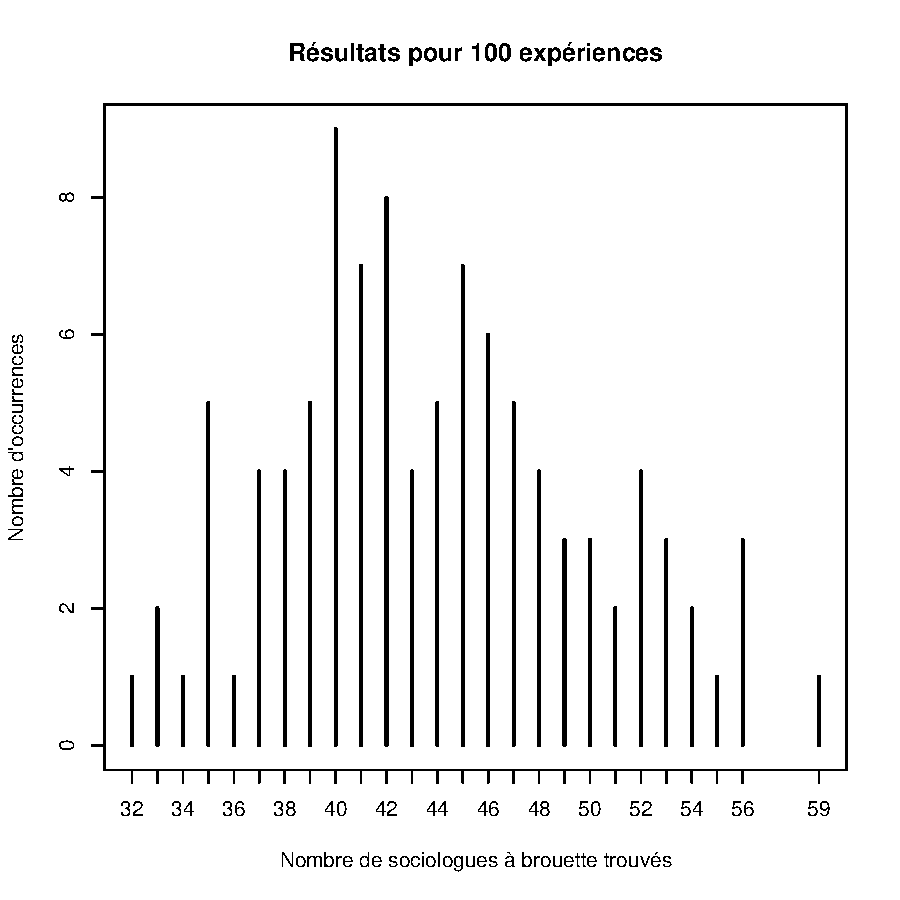
\includegraphics[width=10cm]{images/exp100.pdf}
\end{center}

Ce que nous dit la figure, c'est qu'on a trouvé au minimum 32
et au maximum 59 sociologues à brouettes parmi nos 100 simulations
d'enquêtes, et que le nombre de sociologues à brouette le plus
fréquemment observé est de 40.

L'avantage d'une simulation par ordinateur c'est qu'on peut en faire
facilement autant qu'on veut. On vient d'en faire 100, on va
maintenant en faire 1\,000, 10\,000, 100\,000 et 1\,000\,000. Les
résultats sont indiqués figure~\vref{simexp}.

\begin{figure}
  \begin{center}
    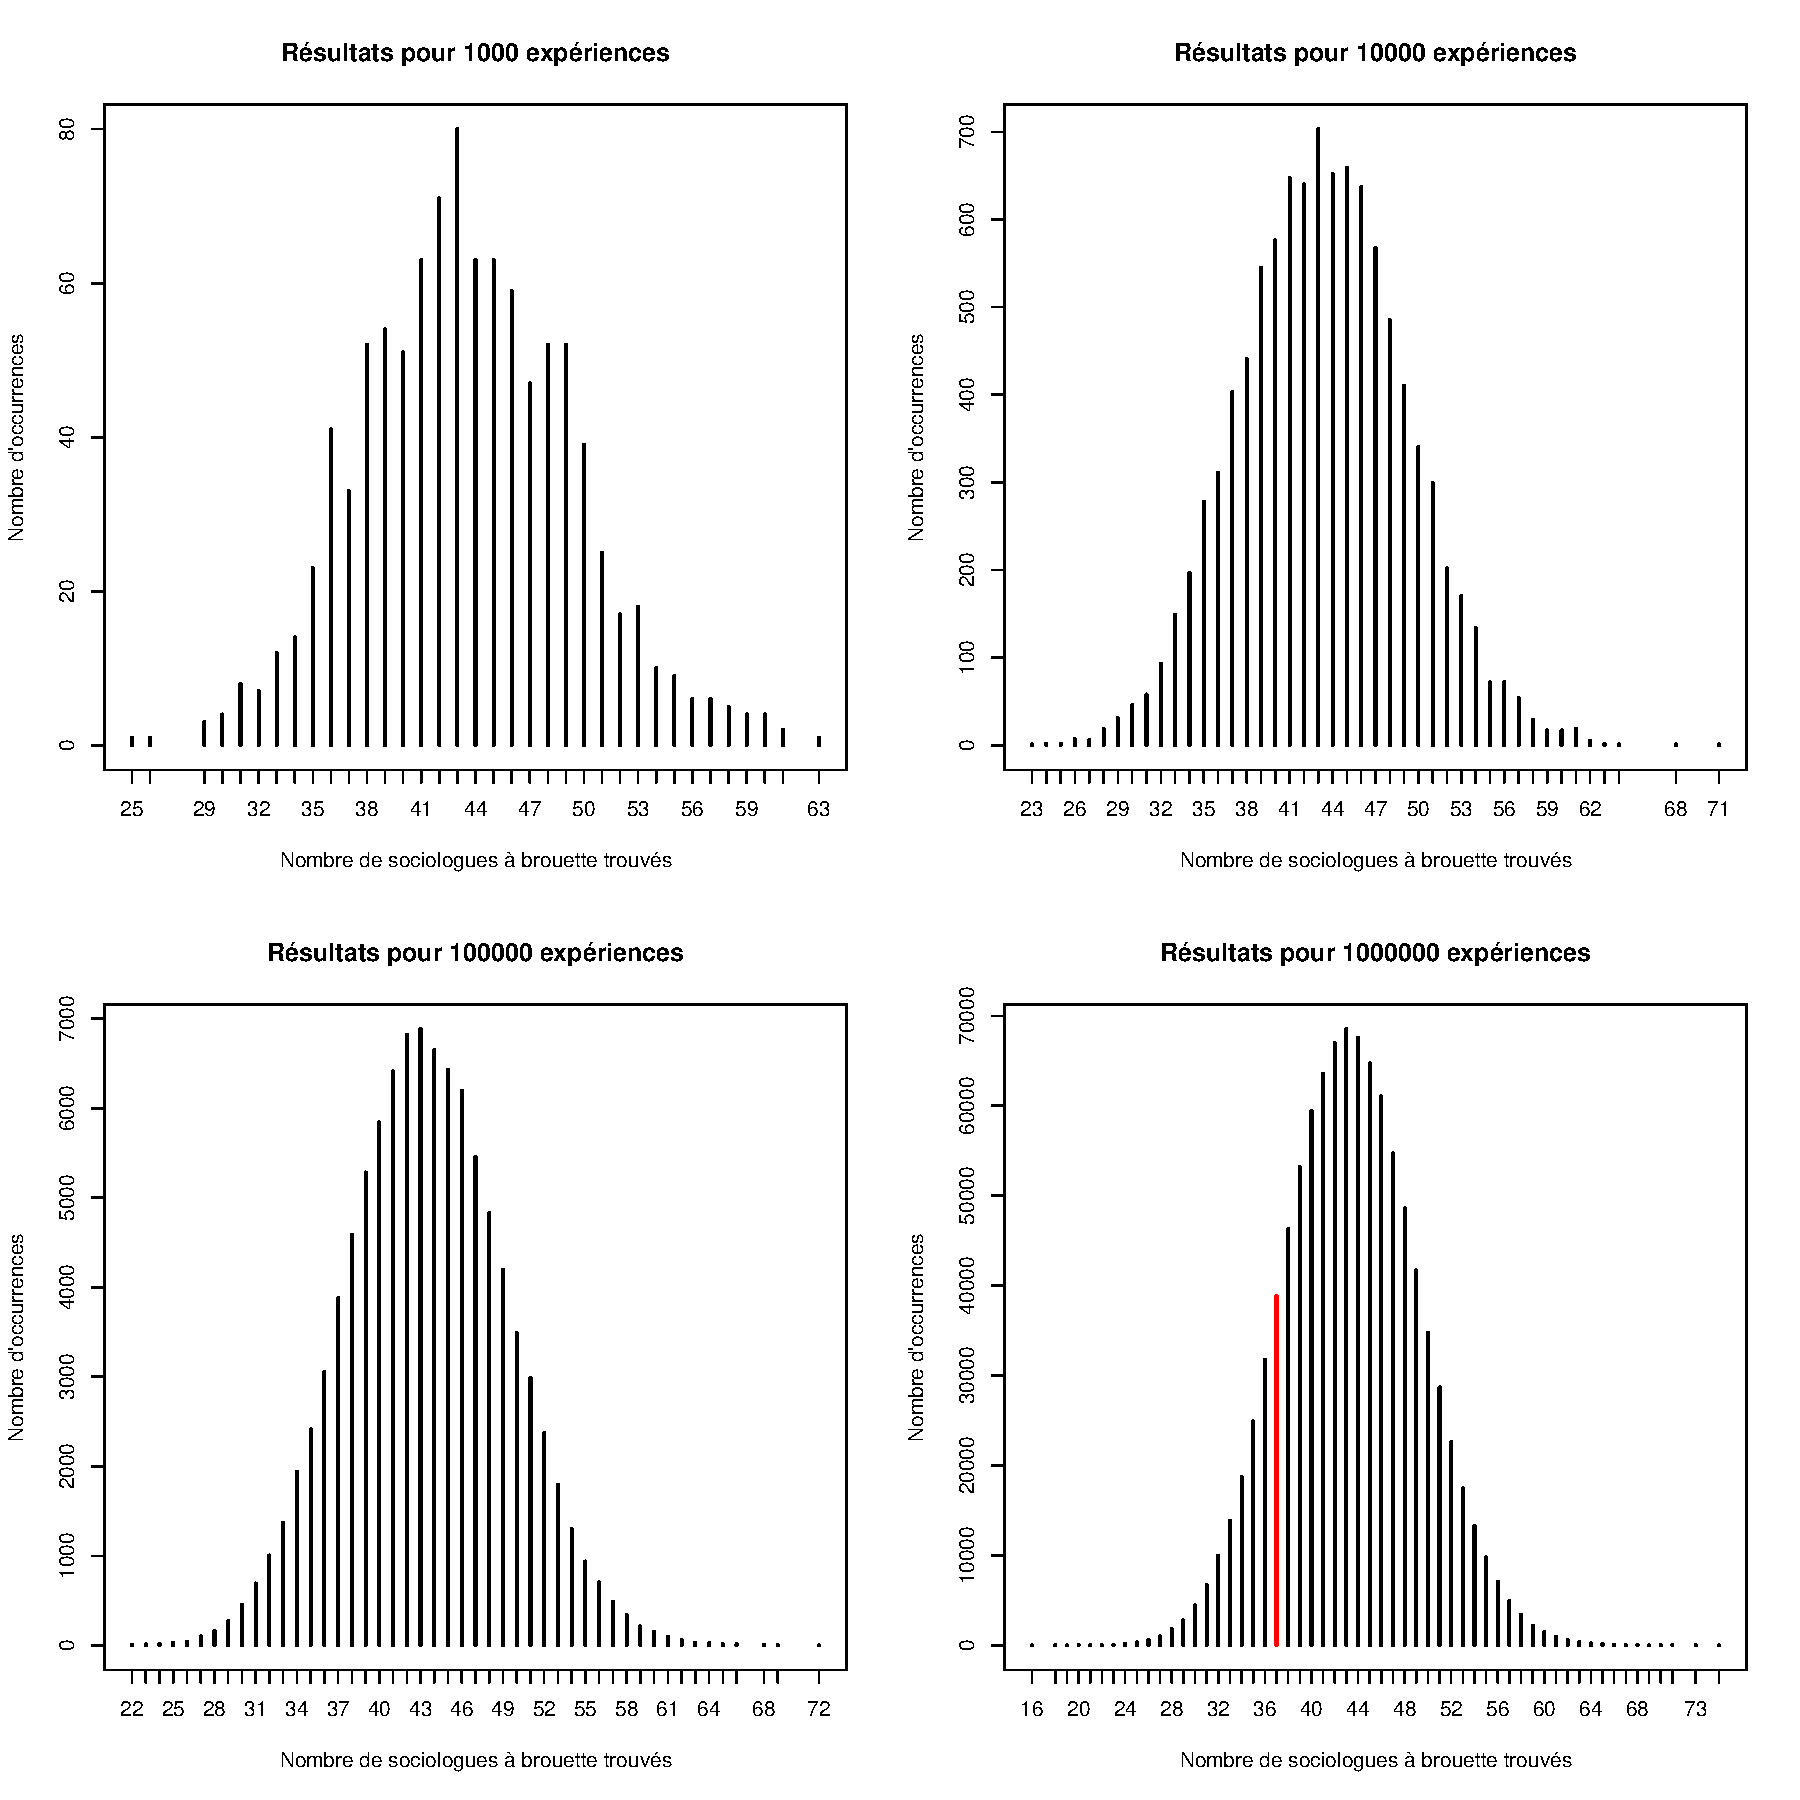
\includegraphics[width=15cm]{images/exp1000_10000_100000.pdf}
  \end{center}
  \caption{Simulation du tirage de sociologues à brouette}
  \label{simexp}
\end{figure}

Que constate-t-on~? d'abord la forme de la répartition semble se
stabiliser avec le nombre de tirages, pour atteindre une forme qui
rappelera sans doute quelque chose à ceux qui ont subi quelques cours
de statistiques durant leurs études. En gros, plus on fait
d'expériences et plus on observe que les résultats ressemblent à la
fonction de densité d'une loi normale (ou courbe de Gauss). Le maximum
semble être atteint pour la valeur 43. Or, on remarquera que les
effectifs théoriques que nous avons calculés s'élèvent justement à
43,4. C'est normal, car les effectifs théoriques sont ceux qu'on a la
plus grande probabilité de trouver sous l'hypothèse d'indépendance.

Soit, voilà une bien jolie courbe. Mais cela ne répond toujours pas à
notre question de savoir si l'écart que nous avons observé est
\og important \fg{} ou non.

Pour cela nous pouvons regarder où se trouve l'effectif observé dans
notre \og vraie \fg{} enquête, c'est-à-dire 37, dans le dernier graphique
de la figure~\ref{simexp}. Pour éviter la survenue d'une presbytie
trop précoce, nous avons pris la peine de surligner la barre du
graphique incriminée en rouge.

Le nombre de fois où on a trouvé 37 s'élève en fait à 38\,806. Si on
ramène à notre million d'expériences cela signifie qu'on a 3,9 chances
sur 100 de trouver un tel résultat sous l'hypothèse d'indépendance des
deux variables. En pratique, la probabilité associée à la seule valeur
37 nous intéresse en fait assez peu~: ce qui nous intéresse c'est de
savoir si 37 est une valeur \og significativement petite \fg{} ou
pas. Donc ce qu'on cherche, ce n'est pas la probabilité d'obtenir
exactement 37, mais plutôt celle d'obtenir 37 \textit{ou moins}.

Ici, on obtient une valeur inférieure ou égale à 37 dans 155\,360 cas
sur un million, soit une probabilité de 15,5 chances sur 100. Ça n'est
pas énorme, mais pas non plus négligeable.

Reformulons ce que nous venons de dire~: si obtient 37 en valeur
observée, il y a 15,5 chances sur 100 que cette valeur soit due au
hasard, c'est-à-dire au biais d'échantillonnage.

Reformulons encore~: si on observe un effectif de 37 et qu'on affirme
qu'il y a un lien entre le fait d'être sociologue et le fait d'avoir
une brouette, on a 15,5 chances sur 100 de se tromper. Est-ce que
c'est beaucoup ou pas~? La statistique n'a pas de réponse à cette
question. Par convention, elle fixe cependant un \og seuil de
significativité \fg{} qui est en général à 5 chances d'erreur sur 100
(c'est le fameux \og significatif au seuil de 5~\% \fg{}). Ce n'est qu'une
convention, mais à défaut d'être mathématique elle a pour elle le fait
que presque tout le monde l'utilise.

Qu'avons nous fait ici~? Nous avons montré qu'on peut, par simulation,
arriver à calculer la probabilité d'obtenir un effectif observé au
plus égal à une certaine valeur sous l'hypothèse d'indépendance. La
statistique ne nous permet pas de dire si une valeur observée est
significativement plus petite ou significativement plus grande
\textit{en soi}, mais elle permet d'estimer une probabilité d'observer
cette valeur dans le cas où les deux variables sont indépendantes.


\section{\chidpdf partiels et \chidpdf du tableau}
\label{ssec-chidpartiels}

Nous venons donc de voir comment, par simulation, on pouvait essayer
de déterminer si les variations observées à l'échelle d'une cellule
ont peu ou beaucoup de chances d'être dues au hasard, ou plus
précisément au biais d'échantillonnage. Il nous reste à voir la même
chose, mais cette fois au niveau du tableau tout entier.

Intuitivement\footnote{En fait ce n'est pas intuitif du tout, mais
  l'expression \textit{intuitivement} permet à l'auteur d'éviter de
  fournir de nouvelles explications laborieuses tout en donnant
  l'impression que pour lui tout ça c'est quand même vachement simple
  et naturel.},  pour passer de la case du tableau au tableau tout
entier, on aurait envie de faire la somme de tous les écarts observés
dans chaque case pour obtenir une sorte d'écart global à
l'indépendance à l'échelle du tableau. Et bien c'est une excellente
idée que vous avez là, et je vous en félicite, mais comme d'habitude
il y a encore une ou deux subtilités dont il va falloir tenir compte.

Tout d'abord, si on essaie immédiatement de faire la somme des écarts
du tableau \vref{ecarts}, on obtient tout aussi
immédiatement\ldots 0~! Si cela ne vous semble pas logique, c'est que
vous n'avez pas lu assez attentivement le paragraphe causant des
contraintes sur les marges, \vpageref{contrmarges}. C'est donc
l'occasion de vous resservir un café ou un jus de tomates et de
reprendre la lecture de ce passionnant passage.

Faire la somme, c'est donc une bonne idée, mais il faut tenir compte
du fait que certains écarts sont positifs et d'autres négatifs et que
tout ça finit par s'annuler. On pourrait s'en sortir en faisant la
somme de la valeur absolue de chaque écart (c'est-à-dire en
transformant les écarts négatifs en écart positif), mais les
statisticiens, souvent d'humeur un peu chafouine, préfèrent utiliser
le carré des écarts, ce qui revient à peu près au même dans la mesure
où le carré d'un nombre est toujours positif\footnote{Le choix de
  passer les écarts au carré s'explique aussi sans doute par le fait
  qu'il permet de distendre les écarts entre les valeurs et de
  faciliter certains calculs.}.

Il reste une deuxième subtilité à prendre en compte, que nous
comprendrons mieux en regardant directement le tableau~\ref{ecarts}.
Si nous regardons la case des sociologues sans brouette, nous
constatons un écart de 6,4. Si on regarde celle des archéologues avec
brouette, on obtient un écart de 3,9. Spontanément on pourrait vouloir
comparer les deux valeurs en affirmant que l'écart est plus grand chez
les sociologues sans brouette que chez les archéologues avec
brouette. Mais il faut tenir compte d'une chose~: les effectifs
théoriques ne sont pas du tout les mêmes dans les deux cases, puisque
nous avions 58,7 sociologues sans brouette attendus contre 8
archéologues avec brouette. Or, un écart de 6 sur une valeur de
référence de 58 semble tout de suite moins importante qu'un écart de
presque 4 sur une valeur de référence qui vaut 8\ldots

En additionnant les écarts de toutes les cases sans tenir compte des
effectifs de référence auxquels ces écarts se rapportent, on risque
donc de mélanger des choux, des carottes, des pommes de terre et des
betteraves. Tout ça peut faire une très bonne soupe (surtout si on
enlève les betteraves), mais du point de vue mathématique le mélange
est assez indigeste.

Pour éviter de boire le potage, on va donc effectuer une opération
assez courante en statistiques, et qu'on nomme
\textit{standardisation}, ce qui signifie qu'on va tout rapporter à
une même échelle, ce qui va permettre de pouvoir travailler sur des
choses comparables entre elles. En pratique, on va diviser la valeur
des écarts par celle des effectifs théoriques correspondant.

\paragraph{Récapitulons} Nous avons notre tableau d'effectifs
observés, notre tableau d'effectifs théoriques. Nous pouvons à partir
de là calculer les écarts entre les deux, mais pour raisonner à
l'échelle du tableau entier nous devons rendre les écarts comparables
en tenant compte d'une part de leur signe (en les élevant au carré) et
d'autre part du fait qu'ils ne se rapportent pas aux mêmes effectifs
de départ (en les divisant par les effectifs théoriques). On va donc
calculer un nouveau tableau dont les cases contiennent la valeur
suivante~:

$$\frac{ ( \text{Effectif observé} - \text{Effectif théorique} )^2}{\text{Effectif théorique}}$$

Cette valeur est appelée le \textit{\chid partiel} de la case du
tableau. Dans notre exemple, on obtient le tableau suivant~:

\begin{table}[H]
  \begin{center}
    \begin{tabular}{lrrr}
      \toprule
      & Sociologue & Banquier & Archéologue\\
      \midrule
      Avec brouette &  0,93 & 0,18 & 1,91\\
      Sans brouette &  0,68 & 0,12 & 1,41\\
      \bottomrule
    \end{tabular}
    \caption{\chid partiels (arrondis)}
    \label{chidpart}
  \end{center}
\end{table}

\textit{Alléluia~!} Nous avons enfin de beaux écarts bien positifs et bien
standardisés, que nous allons pouvoir additionner tous ensemble dans
la joie et l'allégresse. Ce faisant, nous obtenons la fort jolie valeur
de 5,2402, qui n'est rien d'autre que la valeur du \chid pour notre
tableau croisé.

Passée l'euphorie bien compréhensible due à la beauté de ce résultat
arraché à grand renfort d'empilements successifs de subtilités
statistiques et de verres de jus d'artichaut vides dans l'évier de la
cuisine, nous devons néanmoins nous rendre à l'évidence~: 5,2402,
c'est magnifique, mais nous sommes encore et toujours confrontés à la
même question~: c'est beaucoup ou c'est pas beaucoup~?

Avant de répondre, nous allons devoir tenir compte d'une dernière
subtilité statistique. Ne vous inquiétez pas si ce genre de phrase
commence à générer chez vous une certaine lassitude. Mais regardez
là-bas au fond, ne voyez vous pas une faible lueur apparaître dans
l'obscurité~? Le bout du tunnel n'est pas loin, et vous devriez
l'atteindre encore plus facilement en reprenant un grand verre de
nectar d'avocat.



\section{Les degrés de liberté}
\label{ssec-ddl}

La dernière chose dont nous devons tenir compte pour obtenir le
résultat définitif de notre test porte le doux nom de \textit{degré de
liberté}. L'appellation ne manque pas de charme, mais la notion
qu'elle recouvre n'est pas forcément la plus intuitive qui
soit\footnote{L'auteur l'affirme d'autant plus facilement qu'elle est
  loin de l'être pour lui-même et que ça fait un moment qu'il se
  demande comment il va bien pouvoir essayer d'expliquer ce machin.}.

En fait, la notion de degrés de libertés dans le cas du test du \chid
d'indépendance d'un tableau croisé signifie que la valeur calculée du
\chid pour ce tableau doit être rapportée au nombre de colonnes et de
lignes du tableau en question.

Pour tenter de comprendre, reprenons une célèbre enquête menée auprès
de 100 professeurs agrégés, 50 en lettre modernes et 50 en lettres
classiques, auxquels on a demandé leur style musical préféré. On fait
l'hypothèse que les deux variables sont indépendantes. On aurait alors
obtenu, par exemple, le tableau suivant~:

\begin{center}
  \begin{tabular}[!h]{lrr> {\itshape}r}
    \toprule
    & Lettres classiques & Lettres modernes & Total\\
    \midrule
    Hip-hop & 20 & 20 & 40 \\
    Métal & 30 & 30 & 60\\
    \textit{Total} & 50 & 50 & 100 \\
    \bottomrule
  \end{tabular}
\end{center}

Imaginons maintenant que l'enquête ait distingué des
sous-genres musicaux à l'intérieur des catégories \textit{Hip-hop}
et \textit{Métal}~:

\begin{center}
  \begin{tabular}[!h]{lrr> {\itshape}r}
    \toprule
    & Lettres classiques & Lettres modernes & Total\\
    \midrule
    Urban Street Gangsta Rap & 5 & 5 & 10 \\
    Funky Groovy Soul & 15 & 15 & 30 \\
    Industrial Death Metal & 10 & 10 & 20 \\
    Gothic Hard Rock & 20 & 20 & 40 \\
    \textit{Total} & 50 & 50 & 100 \\
    \bottomrule
  \end{tabular}
\end{center}

Maintenant, imaginons qu'un premier agrégé de lettres classiques n'ait
pas entendu la sonnerie du téléphone au moment où notre enquêteur
l'appelait car il écoutait le dernier \textit{Dr. X and the freakin'
  street boyz} à plein volume pendant qu'il travaillait sur une
nouvelle traduction de l'\textit{Ancien testament}. Et que du coup
c'est un autre agrégé de lettres classiques qui a été enquêté, car
celui-ci avait coupé le son de \textit{Sexy groovy funky girlz} pour
pouvoir écouter les commentaires du match Lorient - Valenciennes.

Dans le cas de notre deuxième enquête, ceci a une conséquence claire~:
l'effectif de la case \textit{Lettres classiques} - \textit{Urban
  Street Gangsta Rap} perd un enquêté, au profit de la case
\textit{Lettres classiques} - \textit{Funky Groovy Soul}. Mais dans le
cas de notre première enquête, cet événement n'a aucune influence~:
dans les deux cas on reste dans la case \textit{Lettres classiques} -
\textit{Hip-hop}.

Moralité~? Plus il y a de cases dans le tableau, plus les données sont
susceptibles de varier aléatoirement et donc plus elles sont sensibles
au biais d'échantillonnage.

\paragraph{Version mathématique} D'un point de vue mathématique, cette
notion de \og plus grande sensibilité au biais d'échantillonnage \fg{} est
fortement liée aux contraintes sur les marges.

Pour essayer de comprendre, regardons le premier tableau~: de par les
contraintes sur les marges, je sais quels doivent être mes totaux en
lignes et en colonnes. Maintenant fixons l'effectif de la première
case du tableau (20 dans l'exemple donné). Comme je sais que le total
de la première ligne vaut 40, j'en déduis immédiatement la valeur de
la deuxième case de la première ligne. Et comme je connais aussi les
totaux en colonne, je peux aussi en déduire les valeurs des cases de
la deuxième ligne. En fait, dès que je connais la valeur d'une des
cases, je connais celles de l'ensemble du tableau. On peut donc
considérer que toute la variabilité possible du tableau est contenue
dans une seule case.

Regardons maintenant le deuxième tableau. Si je fixe la première case,
je peux calculer l'effectif de la deuxième case de la première ligne,
mais pas plus. En fait, pour pouvoir reconstruire l'ensemble du
tableau, j'ai besoin de connaître les effectifs de trois cases.

De manière plus générale, le nombre de cases d'un tableau pouvant
varier \og librement \fg{} dans un tableau avec contraintes sur les marges
est toujours égal à~:

$$(\text{Nombre de lignes} - 1) \times (\text{Nombre de colonnes} -
1)$$

Et c'est précisément avec cette formule qu'on calcule le nombre de
\textit{degrés de liberté} d'un tableau\footnote{Les logiciels qui
  appliquent le test du \chid indiquent en général le nombre de degrés
  de liberté du tableau. En général la notation utilisée est
  \textit{ddl} pour les logiciels francophones, et \textit{df} pour
  les anglophones.}.


\section{Le calcul final}
\label{ssec-calcp}

Bien, nous avons désormais d'un côté la valeur du \chid pour notre
tableau, et de l'autre son nombre de degrés de libertés.

Rappelez-vous ce que nous avions fait dans la
section~\vref{secvarcel}~: nous avions réussi à calculer, pour une
cellule de tableau, la probabilité d'obtenir un effectif donné sous
l'hypothèse d'indépendance. Ce calcul avait été obtenu en faisant
toute une série de simulations informatiques. On pourrait procéder de
la même manière à l'échelle de l'ensemble du tableau, mais on se
heurte vite à deux obstacles~:
\begin{enumerate}
\item C'est plus compliqué.
\item Les ordinateurs n'existaient pas quand le test du \chid a été inventé.
\end{enumerate}

La statistique va donc nous permettre de déterminer directement le
même résultat qu'à l'échelle de la cellule, mais sans avoir à
effectuer de simulations\footnote{Les ordinateurs et les algorithmes
  actuels rendent cependant possibles l'utilisation de simulation, ce
  qui est peut être très utile dans certains cas. On en reparlera dans
  le cas où les effectifs théoriques sont considérés comme trop
  faibles, voir section~\vref{ssec-efffaibles}.} et en utilisant des
raisonnements mathématiques. Elle va ainsi nous permettre de
déterminer immédiatement quelle est la probabilité d'obtenir le \chid
observé sur notre tableau compte tenu du nombre de degrés de libertés
et sous l'hypothèse d'indépendance\footnote{Plus précisément, ce que
  nous dit la statistique c'est que la valeur du \chid calculé pour un
  tableau donné sous l'hypothèse d'indépendance des lignes et des
  colonnes tend vers une loi du \chid au nombre de degrés de libertés
  correspondant à celui du tableau.}.

Pour être un peu plus concret, reprenons notre exemple des sociologues
à brouettes. À partir du tableau~\vref{chidpart}, nous avions déduit
que la valeur de notre \chid était de 5,2402. Du fait que le tableau
en question a 2 lignes et 3 colonnes, nous en déduisons que son nombre
de degrés de libertés vaut $(2-1) \times (3-1) = 2$. Et ce que notre
logiciel favori va nous indiquer\footnote{Auparavant les
  statisticiens, qui devaient connaître des week-end longs et pluvieux
  plus fréquemment que la moyenne, s'amusaient à rechercher ces
  informations dans des tables\ldots}, c'est que la probabilité
d'observer un tel résultat compte tenu de l'hypothèse d'indépendance
s'élève à 0,0728. C'est le fameux $p$.

\section{Interprétation du $p$}

L'interprétation de ce $p$ n'est pas si simple, et on peut vite lui faire dire
des choses qu'il ne peut pas dire\footnote{Ce qui était le cas, honte à moi,
  dans de précédentes versions de ce document...}. En fait il n'y a qu'une
seule interprétation rigoureuse~:

\begin{quote}
  \emph{Le $p$, c'est la probabilité d'obtenir une statistique du \chid au
    moins aussi grande que celle obtenue, sous l'hypothèse d'indépendance des
    lignes et des colonnes du tableau croisé.}
\end{quote}

Voilà, c'est tout. 

Bien, mais que fait-on à partir de là~? Et bien la statistique classique propose la
démarche suivante~: on fixe un seuil à l'avance. Si le $p$ obtenu est
inférieur à ce seuil, alors on peut rejeter l'hypothèse d'indépendance et
estimer qu'il y a un lien entre les lignes et les colonnes de mon tableau. Si
le $p$ obtenu est supérieur à ce seuil, alors on ne peut pas rejeter cette
hypothèse d'indépendance.

En général, le seuil le plus couramment utilisé est le fameux seuil des 5~\%,
ou $p=0.05$. 


Le test du \chid, c'est donc~:

\begin{itemize}
\item se placer sous l'hypothèse d'indépendance des lignes et des colonnes de
  mon tableau croisé
\item calculer les effectifs du tableau théorique obtenu sous cette hypothèse
  d'indépendance
\item calculer la statistique du \chid du tableau, qui est une mesure de la
  <<~distance~>> entre le tableau observé et le tableau théorique sous
  l'hypothès d'indépendance
\item en déduire (par approximation mathématique ou par simulation) la
  probabilité $p$ d'obtenir une distance entre les deux tableaux au moins
  aussi grande que celle obtenue
\item si le $p$ obtenu est inférieur à un seuil défini à l'avance (en général
  $p=0,05$), alors on peut rejeter l'hypothèse d'indépendance des lignes et
  des colonnes
\end{itemize}

\textit{Et ça n'est rien d'autre que cela~!}

En particulier, les interprétations suivantes du $p$ ne sont \textbf{pas}
correctes~:

\begin{itemize}
\item \sout{le $p$, c'est la probabilité de se tromper quand on rejette
    l'hypothèse d'indépendance. Si $p=0,05$ j'ai donc 5 chances sur 100 de me
    tromper.}
\item \sout{le $p$ c'est la probabilité que l'hypothèse d'indépendance soit
    vraie.}
\item \sout{si le $p$ est supérieur à 0,5, alors je peux accepter l'hypothèse d'indépendance.}
\end{itemize}



\section{En résumé}

La section qui précède a été longue et fastidieuse. Les détails du
calcul ne sont là que pour comprendre la démarche et faciliter
l'interprétation, les calculs eux-mêmes étant mis en \oe{}uvre par un
logiciel approprié.

\begin{enumerate}
\item Le \chid d'un tableau représente l'écart entre la répartition
  observée dans ce tableau et celle qu'on observerait si les lignes et
  les colonnes de ce tableau étaient indépendantes, c'est-à-dire, si
  le fait d'appartenir à une modalité d'une des deux variables
  croisées n'avait aucun influence sur la modalité d'appartenance de
  la deuxième variable.
\item Le nombre de degrés de libertés dépend du nombre de lignes et de
  colonnes d'un tableau.
\item Avec les deux valeurs précédentes, on peut estimer la
  probabilité $p$ d'obtenir un écart au moins aussi grande entre mon tableau
  observé et le tableau théorique dans le cas où lignes
  et colonnes sont indépendantes. 
\item Un seuil de significativité est fixé pour le $p$, par exemple à 0,05. Si
  le $p$ est inférieur à ce seuil, alors on rejette l'hypothèse d'indépendance
  et on considère qu'un lien existe entre les deux variables. Sinon, le test
  ne nous permet pas de rejeter cette hypothèse d'indépendance.
\end{enumerate}

Nous allons maintenant enfin pouvoir sortir de cette partie théorique
aussi distrayante que l'observation d'un escargot par temps sec pour
aborder des exemples plus concrets d'utilisation du test et
d'interprétation des résultats.


\chapter{Interprétation}
\label{sec-interp}


\section{Résumé des épisodes précédents}

Pour ceux qui n'auraient pas voulu lire les sections précédentes, ceux
qui auraient craqué en cours de route, ou ceux qui auraient ressenti
le besoin de se reposer un moment avant d'attaquer la suite en faisant
deux ou trois semaines de stage de méditation dans un monastère
bouddhiste, voici un récapitulatif des idées à bien assimiler pour
comprendre ce qui suit.

Le test du \chid vise à tester l'hypothèse d'indépendance des lignes
et des colonnes d'un tableau croisé. Cette hypothèse signifie que~:
\begin{enumerate}
\item Le fait d'appartenir à l'une des modalités de la première
  variable n'a aucune influence sur la modalité d'appartenance de la
  seconde.
\item Les pourcentages lignes du tableau croisé sont les mêmes pour
  toutes les lignes.
\item Les pourcentages colonnes du tableau croisé sont les mêmes pour
  toutes les colonnes.
\end{enumerate}

Le test du \chid se base sur la valeur du \chid du tableau, qui est
une mesure de l'écart entre le tableau observé et le tableau qu'on
aurait obtenu si les variables étaient parfaitement indépendantes, et
sur le nombre de degrés de liberté du tableau, qui dépend du nombre de
lignes et de colonnes.

À partir de ces deux données, le test donne une valeur $p$ qui est la
probabilité d'obtenir un écart au moins aussi grand que celui observé sous
l'hypothèse d'indépendance de mes lignes et de mes colonnes.

Si le $p$ est inférieur à un seuil fixé à l'avance (bien souvent 0,05, ou
5~\%), on dit que le test est significatif et qu'on peut rejeter l'hypothèse
d'indépendance des lignes et des colonnes du tableau.

\section{Valeur du \texorpdfstring{$p$}{p}}
\label{ssec-valp}


Le tableau suivant est, pour une fois, tiré de données réelles, en
l'occurrence celles de l'enquête \textit{Histoire de vie} réalisée en
2003 par l'INSEE\footnote{Dans ces exemples on s'est contenté des
  données brutes et on n'a pas utilisé la pondération donnée par
  l'INSEE.}. Il croise le fait d'avoir été élevé par sa mère seule
jusqu'à 18 ans par la catégorie socio-professionnelle du père en 6
postes.


\begin{table}[H]
  \begin{center}
    \small
    \begin{tabular}[!h]{lrrrrrr}
      \toprule
      & Agriculteur & Indépendant & Cadre & Intermédiaire & Employé & Ouvrier\\
      \midrule
      Élevé par sa mère seule & 22 & 50 & 60 & 57 & 50 & 161 \\
      Autre & 990 & 801 & 572 & 800 & 690 & 2861 \\
      \bottomrule
    \end{tabular}
  \end{center}
  \caption{Croisement de la CS du père avec le fait d'avoir été élevé
    seul par sa mère}
  \label{cselev}
  \normalsize
\end{table}

Le \chid vaut 44,63, le nombre de degrés de libertés est 5, $p$ vaut
0,00000001726.

On peut donc rejeter l'hypothèse d'indépendance sans crainte, le $p$ est
extrêmement faible et largement au-dessous du seuil de 0,05. La
catégorie sociale d'appartenance du père a une influence sur le fait
d'avoir été ou non élevé par sa mère seule.

Le tableau qui suit croise le fait de pratiquer ou non le football et
le sentiment d'appartenir ou non à une classe sociale~:

\begin{center}
  \begin{tabular}[!h]{lrr}
    \toprule
     & Pratique le football & Ne pratique pas le football\\
    \midrule
    Sentiment d'appartenance & 93 & 3921 \\
    Pas de sentiment d'appartenance & 92 & 4165 \\
    Ne sait pas & 1 & 131 \\
    \bottomrule
  \end{tabular}
\end{center}

Le \chid vaut 1,5448, le nombre de degrés de libertés est 2, $p$ vaut
0,4619.

L'hypothèse d'indépendance entre les deux variables ne peut donc \textit{a
priori} pas être rejetée, on ne peut pas établir de lien entre les deux
variables.


\section{Le test du \chidpdf est symétrique}
\label{ssec-sym}

Comme on a déjà eu l'occasion de le souligner\footnote{Mais vous aurez
remarqué que ce document ne recule pas devant une certaine dose de
répétitions, mais si celle-ci frise parfois le radotage.}, les
lignes et les colonnes d'un tableau croisé sont interchangeables.
Vous pouvez donc échanger vos deux variables, le résultat du test
sera toujours exactement le même.

Ceci signifie notamment que le tableau n'a pas en lui-même de
\textit{sens de lecture}~: c'est notre connaissance de l'objet étudié
qui nous fait dire \og le sexe a une influence sur le fait de préférer
la choucroute ou les brocolis \fg{} et non pas \og le fait de préférer
la choucroute ou les brocolis a une influence sur le sexe \fg{}.

Ce que le \chid nous dit, c'est \og les deux variables sont
dépendantes \fg{}. Ce qu'il ne nous dit pas, c'est \og la variable Y est
dépendante de la variable X \fg{}. Le fait de considérer une variable
comme ayant une influence sur une autre relève de l'interprétation et
de l'analyse. Cela se traduit en général par le choix d'utiliser les
pourcentages lignes ou les pourcentages colonnes dans la lecture du
tableau.

Si on reprend l'exemple du tableau~\ref{cselev}, l'interprétation va
naturellement dans le sens d'une influence de la catégorie sociale du
père sur le fait d'avoir été élevé seul par sa mère, et non
l'inverse. Ceci se traduit par l'utilisation de pourcentages colonnes
pour l'analyse du tableau~:

\begin{table}[H]
  \begin{center}
    \footnotesize
    \begin{tabular}[!h]{lrrrrrr> {\itshape}r}
      \toprule
      & Agriculteur & Indépendant & Cadre & Intermédiaire & Employé &
      Ouvrier & Ensemble \\
      \midrule
      Élevé par sa mère seule & 2,2~\% & 5,9~\% & 9,5~\% & 6,7~\% & 6,8~\% & 5,3~\% & 5,6~\% \\
      Autre & 97,8~\% & 94,1~\% & 90,5~\% & 93,3~\% & 93,2~\% & 94,7~\% & 94,4~\%\\
      \textit{Total} & 100,0~\%  & 100,0~\% & 100,0~\% & 100,0~\% &
      100,0~\% & 100,0~\% & 100,0~\% \\
      \bottomrule
    \end{tabular}
    \normalsize
  \end{center}
\end{table}

C'est grâce aux pourcentages colonnes qu'on peut approfondir l'analyse
du tableau au-delà de la seule existence ou non d'une dépendance entre
les variables. Ils nous permettent en effet, par exemple, de constater
que seuls 2,2~\% des enquêtés dont le père est agriculteur ont été
élevé seuls par leur mère, contre 9,5~\% de ceux dont le père est
cadre, la moyenne pour l'ensemble des enquêtés étant de
5,6~\%\footnote{Cette analyse sera grandement facilitée et
  statistiquement validée par l'utilisation des \textit{résidus}, voir
section~\vref{sec-residus}.}.



\section{Le test du \chidpdf dépend du découpage en modalités}
\label{ssec-modal}

Dans ce qui précède on a pu dire indifféremment que le test du \chid
portait sur l'indépendance des lignes et des colonnes d'un tableau
croisé, ou bien sur les deux variables d'un tableau croisé. En fait,
la première formulation est plus rigoureuse, car la deuxième tend à
masquer le fait que la manière dont chacune des deux variables est
découpée en modalités joue un rôle considérable dans la valeur finale
du test.

Il semble parfois contre-intuitif d'imaginer que la manière dont on
code, découpe ou regroupe une variable en classes ou en modalités
puisse influencer sa dépendance ou son indépendance vis-à-vis
d'autres variables. Si on tient compte de la manière dont le \chid est
calculé, cette influence s'explique cependant assez bien~:

\begin{itemize}
\item si on regroupe des modalités existantes ou si on en crée de
  nouvelles, les dimensions du tableau changent, et donc le degré de
  liberté qui lui est associé également. Ceci influence donc la valeur
  finale du $p$~;
\item mais surtout, selon la manière dont on regroupe ou éclate ces
  modalités, on peut masquer des écarts à l'indépendance ou au
  contraire en faire apparaître de nouveaux.
\end{itemize}

Prenons un exemple à nouveau tiré de l'enquête \textit{Histoire de
  vie} en croisant l'âge (découpé en classes) et la variable indiquant
si les types d'émission préférés à la télévision sont les séries et les
feuilletons. Commençons par un découpage en âges assez fin (ici on
donne les pourcentages colonnes)~:

\begin{table}[H]
  \begin{center}
    \footnotesize
    \begin{tabular}[!h]{lrrrrrr> {\itshape}r}
      \toprule
      & 25 et moins & 26-35 & 36-45 & 46-55 & 56-65 & 66 et plus & Ensemble \\
      \midrule
      Oui & 20,4~\% & 9,8~\% & 7,5~\% & 7,5~\% & 8,1~\% & 12,5~\% & 10,2~\% \\
      Non & 79,6~\% & 90,2~\% & 92,5~\% & 92,5~\% & 91,9~\% & 87,5~\% & 89,8~\%\\
      \textit{Total} & 100,0~\%  & 100,0~\% & 100,0~\% & 100,0~\% & 100,0~\% & 100,0~\% & 100,0~\% \\
      \bottomrule
    \end{tabular}
    \normalsize
  \end{center}
\end{table}

Le \chid est extrêmement significatif ($p$ quasiment égal à zéro). On
constate que les séries et les feuilletons sont préférés à la fois par
les plus jeunes et par les plus âgés\footnote{Phénomènes bien connus
  en sociologie des médias et identifiés respectivement sous les noms
  d'\textit{effet Prison break} et d'\textit{effet Derrick}.}.

Imaginons maintenant que la question qui nous intéressait au départ
était de différencier les moins de 55 ans des plus de 55 ans. Nous
aurions alors obtenu le tableau suivant~:

\begin{table}[H]
  \begin{center}
    \footnotesize
    \begin{tabular}[!h]{lrr> {\itshape}r}
      \toprule
      & 55 et moins & 56 et plus & Ensemble \\
      \midrule
      Oui & 10,0~\% & 10,5~\% & 10,2~\% \\
      Non & 90,0~\% & 89,5~\% & 89,8~\% \\
      \textit{Total} & 100,0~\%  & 100,0~\% & 100,0~\% \\
      \bottomrule
    \end{tabular}
    \normalsize
  \end{center}
\end{table}

Avec un \chid plus du tout significatif, puisque le $p$ vaut désormais
0,49~! En regroupant les classes d'âge, on a regroupé des catégories
où la préférence pour les séries était sur-représentée et d'autres où
elle ne l'était pas du tout. Au final, on a construit deux populations
homogènes en regroupant des populations hétérogènes mais opposées.

De manière générale, il est donc préférable de partir avec des
découpages en classes les plus détaillés possibles, pour pouvoir
éventuellement ensuite pouvoir regrouper entre elles des modalités
ayant des profils semblables (identifiés par leurs pourcentages lignes
ou colonnes). Dans notre exemple, on aurait pu regrouper les tranches
d'âge de 36 à 65 ans pour mieux faire ressortir l'opposition entre les
âges intermédiaires et les âges \og extrêmes \fg{}.



\section{Le test du \chidpdf dépend des effectifs}
\label{ssec-depeff}

Dans une étude évidemment très sérieuse réalisée par le ministère de
la Santé, on a voulu étudier le lien entre le degré de calvitie et le
fait d'avoir ou non attrapé un rhume dans les six derniers
mois. On a interrogé un premier échantillon en obtenant les
résultats suivants~:

\begin{table}[H]
  \begin{center}
    \begin{tabular}[!h]{lrr}
      \toprule
      & A eu un rhume & N'a pas eu de rhume \\
      \midrule
      Totalement chauve & 7 & 5 \\
      Partiellement chauve & 4 & 8 \\
      Porte une perruque & 9 & 12 \\
      \bottomrule
    \end{tabular}
  \end{center}
\end{table}

Si on fait les pourcentages lignes, on obtient le tableau suivant~:

\begin{table}[H]
  \begin{center}
    \begin{tabular}[!h]{lrr> {\itshape}r}
      \toprule
      & A eu un rhume & N'a pas eu de rhume & Total\\
      \midrule
      Totalement chauve & 58,3~\% & 41,7~\% & 100~\%\\
      Partiellement chauve & 33,3~\% & 66,7~\% & 100~\% \\
      Porte une perruque & 42,9~\% & 57,1~\% & 100~\% \\
      \textit{Ensemble} & \textit{44,4~\%} & \textit{55,6~\%} & 100~\% \\
      \bottomrule
    \end{tabular}
  \end{center}
\end{table}

Le \chid de notre tableau n'est pas du tout significatif, avec un $p$
de 0,459. Fort déçu, le ministère a décidé de renouveler l'enquête
mais en accordant une rallonge budgétaire qui a permis d'interroger
dix fois plus de personnes, avec les résultats suivants~:

\begin{table}[H]
  \begin{center}
    \begin{tabular}[!h]{lrr}
      \toprule
      & A eu un rhume & N'a pas eu de rhume \\
      \midrule
      Totalement chauve & 70 & 50 \\
      Partiellement chauve & 40 & 80 \\
      Porte une perruque & 90 & 120 \\
      \bottomrule
    \end{tabular}
  \end{center}
\end{table}

Si on calcule les pourcentages lignes de ce nouveau tableau, on
obtient exactement les mêmes que précédemment, car les effectifs de
chaque case ont tous été multipliés par 10.

Par contre, le \chid de ce nouveau tableau est lui devenu très
significatif, avec un $p$ inférieur à 0,001.

Que s'est-il passé~? On vient tout simplement d'observer le fait que
plus les effectifs de notre tableau augmentent, plus les écarts à
l'indépendance observés ont de chances d'être significatifs. Si
j'interroge dix personnes et que j'obtiens six fois \textit{oui} et
quatre fois \textit{non}, je ne peux rien dire. Mais si j'en interroge
10\,000 et que j'obtiens 6\,000 \textit{oui} et 4\,000 \textit{non},
là je peux en conclure quelque chose.

Le \chid est donc extrêmement sensible aux effectifs~: plus ceux-ci
sont élevés, plus la part de variation dans mon tableau due au biais
d'échantillonnage est faible. À écarts de répartition équivalents, on aura
donc une valeur du $p$ plus petite si les effectifs sont plus élevés.

Un \chid non significatif (c'est-à-dire un $p$ supérieur au seuil de
significativité) peut donc signifier soit qu'on ne
peut rejeter l'hypothèse d'indépendance entre les lignes et les
colonnes du tableau (dans le cas où les pourcentages lignes ou
colonnes sont très proches les uns des autres), soit qu'il n'y a pas
indépendance mais que les effectifs dont je dispose ne me permettent
pas d'en être sûr statistiquement (dans le cas où les pourcentages
lignes ou colonnes sont sensiblement différents). Le test ne nous permet pas
de trancher entre les deux possibilités, sauf à refaire une enquête avec des
effectifs plus importants.


\section{Le test du \chidpdf ne mesure pas l'intensité de la dépendance}
\label{sec-intdep}

En fait, ceci découle directement de la section précédente et de la
sensibilité du \chid aux effectifs. Prenons les deux tableaux
suivants~:

\begin{center}
  \hfill
  \begin{minipage}[c]{.46\linewidth}
    \begin{tabular}[!h]{lrr}
      \toprule
      & Rouge & Vert \\
      \midrule
       Rond & 10 & 20 \\
       Carré & 20 & 10 \\
      \bottomrule
    \end{tabular}
  \end{minipage}
  \hfill
  \begin{minipage}[c]{.46\linewidth}
    \begin{tabular}[!h]{lrr}
      \toprule
      & Rouge & Vert \\
      \midrule
      Rond & 100 & 200 \\
      Carré &  200 & 100 \\
      \bottomrule
    \end{tabular}
  \end{minipage}
  \hfill
\end{center}

Si on veut parler de la force de la dépendance entre les deux
variables, on ne peut pas différencier ces deux tableaux~: la
répartition des effectifs entre les cases est la même, les
pourcentages lignes et colonnes sont identiques. Pourtant si dans le
premier cas on a bien un \chid significatif d'une valeur de 5,4 avec
un $p$ de 0,02, dans le second le test devient extrêmement significatif
avec un \chid de 65,34 et un $p$ quasiment égal à zéro.

Le raisonnement ici est exactement le même que dans la section
précédente~: pour une même répartition dans mon tableau, j'ai d'autant
plus de chances d'être significativement éloigné de l'indépendance que
mes effectifs sont importants.

Ce qu'on peut en conclure ici c'est que les valeurs du \chid et du $p$
ne doivent pas être utilisées comme indicateurs de la force du lien de
dépendance entre les variables du tableau croisé. On ne peut donc pas
comparer les résultats du test du \chid pour deux tableaux différents
en en concluant que la dépendance entre les variables serait plus
forte pour l'un que pour l'autre\footnote{Pour être tout à fait
  rigoureux, on pourrait le faire mais seulement quand les deux
  tableaux ont les mêmes dimensions et les mêmes effectifs
  totaux. Mais dans tous les cas on préfère utiliser des indices
  calculés exprès pour, comme le $V$ de Cramer, que nous verrons
  section~\vref{sec-vcramer}.}.

Une autre conclusion est qu'avec des effectifs très importants, les \chid des
tableaux croisés seront quasiment toujours significatifs, puisque même la plus
petite variation de pourcentages pourra devenir significative.

Repartons de l'exemple croisant calvitie et rhume, et imaginons que nous avons
interrogé 10\,000\,000 de personnes, avec le résultat suivant~:

\begin{table}[H]
  \begin{center}
    \begin{tabular}[!h]{lrr}
      \toprule
      & A eu un rhume & N'a pas eu de rhume \\
      \midrule
      Totalement chauve & 6\,700\,000 & 3\,300\,000 \\
      Partiellement chauve & 2\,676\,000 & 1\,324\,000 \\
      Porte une perruque &  671\,000 & 329\,000 \\
      \bottomrule
    \end{tabular}
  \end{center}
\end{table}

Si on fait les pourcentages lignes, on obtient le tableau suivant~:

\begin{table}[H]
  \begin{center}
    \begin{tabular}[!h]{lrr> {\itshape}r}
      \toprule
      & A eu un rhume & N'a pas eu de rhume & Total\\
      \midrule
      Totalement chauve & 67,0~\% & 33,0~\% & 100~\%\\
      Partiellement chauve & 66,9~\% & 33,1~\% & 100~\% \\
      Porte une perruque & 67,1~\% & 32,9~\% & 100~\% \\
      \textit{Ensemble} & \textit{67,0~\%} & \textit{33,0~\%} & 100~\% \\
      \bottomrule
    \end{tabular}
  \end{center}
\end{table}

Les écarts entre les pourcentages ligne sont extrêmement faibles. Et pourtant,
on obtient un \chid de 19,894 pour 2 degrés de liberté, soit un $p =
0.00004786$, très largement en-dessous du seuil de 5~\%. Les effectifs très
importants permettent de rejeter l'hypothèse d'indépendance, même si le lien
entre lignes et colonnes du tableau observé semble très faible. 



\section{Les résidus}
\label{sec-residus}

Les résidus sont une aide à l'interprétation extrêmement utile pour
l'analyse d'un tableau croisé. Pour le dire rapidement, le \chid
indique si les écarts à l'indépendance sont significatifs à l'échelle
du tableau, les résidus, eux, donnent cette indication à l'échelle de
chaque cellule. Leur résultat est en fait très proche de ce que nous
avons effectué dans la section \textit{Variations à l'échelle d'une
  cellule}, \vpageref{secvarcel}.

Dans cette section, nous avions tenté de voir comment on peut, par
simulation, estimer si, à l'échelle d'une case, un écart entre un
effectif observé et un effectif attendu était statistiquement
significatif ou non. Les résidus permettent d'obtenir cette
information pour toutes les cases et donc de déterminer dans quels
sens vont les écarts et où ceux-ci sont significatifs.

D'un point de vue mathématique, il existe deux types de résidus~: les
\textit{résidus de Pearson} et les \textit{résidus de Pearson
  standardisés} (ou ajustés). La différence entre les deux a
relativement peu d'importance, car leur interprétation est semblable. D'un
point de vue calcul et à titre tout à fait indicatif, la formule pour
les résidus de Pearson est la suivante~:

$$\frac{\text{Effectifs observés} - \text{Effectifs
    théoriques}}{\sqrt{\text{Effectifs théoriques}}}$$

La formule des résidus est un tantinet plus complexe\footnote{Pour
  plus d'informations, on pourra se reporter à
  \cite[p.\,81]{Agresti2002}.}, mais l'interprétation est la même dans
les deux cas.

Au final il n'y a que deux choses à retenir~:

\begin{itemize}
\item si un résidu est positif, c'est que les effectifs dans la case
  sont supérieurs à ceux attendus sous l'hypothèse
  d'indépendance. S'il est négatif, c'est que les effectifs observés
  sont inférieurs aux effectifs théoriques~;
\item les résidus correspondant à des écarts statistiquement
  significatifs sont \textit{grosso modo} ceux dont la valeur est
  supérieure à 2 ou inférieure à -2\footnote{Ceci étant dû au fait que
    les résidus tendent à suivre une loi normale centrée réduite.}.
\end{itemize}

Tout cela peut sembler compliqué, mais un exemple permettra de mieux
comprendre de quoi il s'agit. Exemple réel cette fois, tiré toujours
de l'enquête \textit{Histoire de vie}, et pour lequel nous allons
croiser la catégorie sociale et le sentiment d'appartenir à une
classe sociale~:

\begin{table}[H]
  \begin{center}
    \begin{tabular}[!h]{lrrrrrr}
      \toprule
      & Appartient & N'appartient pas & Ne sait pas \\
      \midrule
      Agriculteur & 125 & 194 & 9 \\
      Indépendant & 190 & 300 & 6 \\
      Cadre & 588 & 433 & 9 \\
      Intermédiaire & 842 & 694 & 10 \\
      Employé & 1105 & 1227 & 38 \\
      Ouvrier & 888 & 1024 & 45 \\
      \bottomrule
    \end{tabular}
  \end{center}
\end{table}

Le \chid est extrêmement significatif, avec un $p$ proche de zéro.

On peut regarder les pourcentages lignes~:

\begin{table}[H]
  \begin{center}
    \begin{tabular}[!h]{lrrr}
      \toprule
      & Appartient & N'appartient pas & Ne sait pas \\
      \midrule
      Agriculteur & 38,1~\% & 59,1~\% & 2,7~\% \\
      Indépendant & 38,3~\% & 60,5~\% & 1,2~\% \\
      Cadre & 57,1~\% & 42,0~\% & 0,9~\% \\
      Intermédiaire & 54,5~\% & 44,9~\% & 0,6~\% \\
      Employé & 46,6~\% & 51,8~\% & 1,6~\% \\
      Ouvrier & 45,4~\% & 52,3~\% & 2,3~\% \\
      \textit{Ensemble} & 48,4~\% & 50,1~\% & 1,5~\% \\
      \bottomrule
    \end{tabular}
  \end{center}
\end{table}

Plus le nombre de cases est élevé, plus il devient difficile de lire
le tableau. Regardons ce que valent les résidus (ici les résidus de
Pearson)~:

\begin{table}[H]
  \begin{center}
    \begin{tabular}[!h]{lrrrrrr}
      \toprule
      & Appartient & N'appartient pas & Ne sait pas \\
      \midrule
      Agriculteur & \textbf{-2,7} & \textbf{2,3} & 1,8 \\
      Indépendant & \textbf{-3,2} & \textbf{3,3} & -0,6 \\
      Cadre & \textbf{4,0} & \textbf{-3,7} & -1,7 \\
      Intermédiaire & \textbf{3,4} & \textbf{-2,9} & \textbf{-2,8} \\
      Employé & -1,2 & 1,1 & 0,4 \\
      Ouvrier & -1,9 & 1,4 & \textbf{2,8} \\
      \bottomrule
    \end{tabular}
  \end{center}
\end{table}

Les résidus permettent \og d'orienter le regard \fg{} vers les cases où
les écarts sont statistiquement significatifs. \textit{A priori}, en
regardant ce dernier tableau on peut se rendre compte que le sentiment
d'appartenance à une classe sociale est moins fréquent que la moyenne
chez les agriculteurs et les indépendants, tandis qu'il l'est plus
chez les cadres et les professions intermédiaires. Par ailleurs,
ceux-ci sont moins nombreux que la moyenne à ne pas savoir s'ils
appartiennent ou non à une classe sociale, tandis que les ouvriers
sont un peu plus nombreux que la moyenne à être dans ce cas.

Il y a cependant une chose importante à noter lorsqu'on utilise les
résidus, c'est que ceux-ci mesurent la significativité de l'écart
par rapport aux effectifs théoriques attendus de la case. Ils sont
donc liés à ces derniers~: un écart de 10 quand les effectifs
théoriques étaient de 20 (c'est-à-dire un effectif observé de 30) sera
sans doute significatif, tandis que le même écart de 10 quand les
effectifs théoriques sont de 2\,000 ne le sera pas.

Ainsi, de la même manière que pour le \chid, avoir un résidu très
supérieur à 2 ne signifie pas que l'écart entre effectifs observés et
effectifs théoriques est très élevé. Ceci signifie juste qu'il est
très significativement différent de zéro. Dans notre exemple, si on
regarde la case des ouvriers ne sachant pas s'ils appartiennent ou non
à une classe sociale, on a un résidu supérieur à 2 avec un écart de
\og seulement \fg{} 0,8 points par rapport au profil moyen (2,3~\%
contre 1,5~\%). Encore une fois, c'est en se rapportant aux
pourcentages lignes ou colonnes qu'on peut voir si l'écart au profil
moyen est élevé ou pas.

Résumons~:

\begin{itemize}
\item les résidus indiquent dans quelle case on a des
  sur-représentations (si leur valeur est supérieure à 2) ou des
  sous-représentations (si elle est inférieure à -2) statistiquement
  significatives~;
\item ils orientent le regard vers les cases pour lesquelles on peut
  dire quelque chose, et montrent à l'inverse celles pour lesquelles
  l'écart au profil moyen n'est pas significatif~;
\item en dernier lieu ce sont toujours les pourcentages lignes ou
  colonnes qui permettent de mesurer l'amplitude de cet écart.
\end{itemize}

Les résidus sont donc très utiles pour l'analyse d'un tableau dont
le \chid permet de rejeter l'hypothèse d'indépendance. Ils le seront
d'autant plus que le tableau comporte un grand nombre de cases. Ils
permettent de plus de valider statistiquement les écarts observés à
l'échelle de la case\footnote{Il est dommage que certaines logiciels
  comme \textsf{Modalisa} ne proposent pas le calcul des résidus pour
  les tableaux croisés, même si dans ce cas l'utilisation du PEM
  (pourcentage de l'écart maximum) s'en rapproche
  \cite{Cibois1993pem}.}.


\paragraph{Représentation graphique}

L'utilisation des résidus a un autre avantage, c'est de permettre la
représentation graphique de tableaux croisés incluant les liens entre
les différentes modalités, c'est à dire les cases dans lesquelles les
effectifs observés sont significativement supérieurs ou inférieurs aux
effectifs théoriques.

\begin{figure}
  \begin{center}
    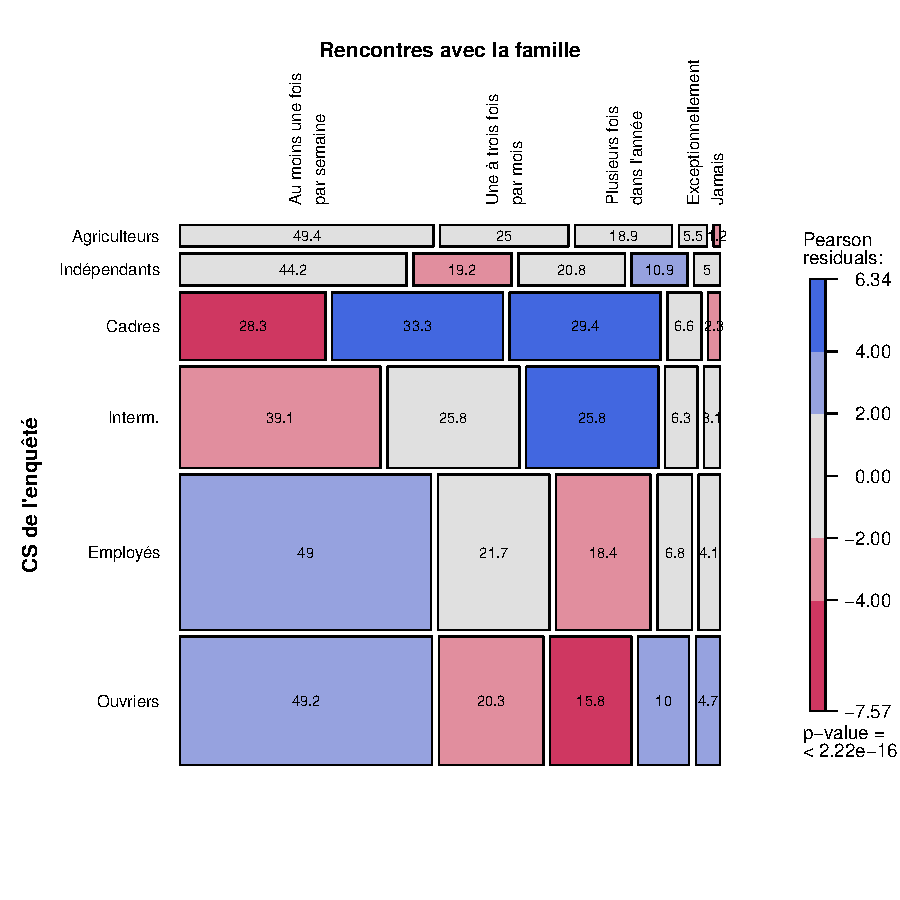
\includegraphics[width=15cm]{images/mosaic.pdf}
  \end{center}
  \caption{Graphique en mosaïque du croisement entre la CS de
    l'enquêté et la fréquence des visites dans la famille}
  \label{fig_mosaic}
\end{figure}

Prenons par exemple la figure~\vref{fig_mosaic}. Elle représente le
tableau croisant, pour l'enquête \textit{Histoire de vie}, la
catégorie professionnelle de l'enquêté et la fréquence de ses visites
à sa famille proche ou éloignée. Ce graphique contient une
représentation visuelle de chaque case construite de la façon
suivante~:

\begin{itemize}
\item la largeur de chaque case est proportionnelle au pourcentage
  ligne correspondant. On a d'ailleurs indiqué dans chaque case la
  valeur de ce pourcentage~;
\item la surface de la case est proportionnelle aux effectifs observés~;
\item la couleur de la case dépend de la valeur du résidu de Pearson
  associé~: bleu si le résidu est significativement positif, rouge
  s'il est significativement négatif, gris s'il n'est pas
  significatif.
\end{itemize}

La lecture de ce type de graphique n'est peut-être pas évidente de
prime abord, mais une fois habitué elle permet de synthétiser de
manière visuelle la quasi-totalité des informations nécessaires pour
l'analyse.

Pour reprendre l'exemple de la figure~\ref{fig_mosaic}, on peut ainsi
voir immédiatement que les employés et les ouvriers ont plus
fréquemment des visites familiales hebdomadaires, tandis que les
cadres et les professions intermédiaires en ont moins souvent. On
remarquera également que le pourcentage est très élevé chez les
agriculteurs (49,4~\%), mais que l'écart n'est pas significatif, sans
doute du fait d'effectifs trop faibles. On peut également remarquer
que les cadres ont plus souvent des fréquences de visite
intermédiaires (plusieurs fois par mois ou par an) tandis que les
ouvriers ont plus souvent des fréquences de visite \og extrêmes \fg{}
(soit hebdomadaires, soit exceptionnelles ou inexistantes).

Ce type de graphique en mosaïque permet donc de faciliter l'analyse,
là encore plus particulièrement dans le cas de tableaux croisés avec
un nombre de cases élevé.


\chapter{Limites}
\label{sec-limites}

\section{Fausse limite~: quand les effectifs théoriques sont trop faibles}
\label{ssec-efffaibles}

Commençons par un exemple. Soit le tableau croisé suivant, qui
s'intéresse au fait de gagner ou non au Loto selon qu'on possède un
trèfle à quatre feuilles, un fer à cheval ou aucun des deux~:


\begin{table}[H]
  \begin{center}
    \begin{tabular}[!h]{lrr}
      \toprule
      & Perdant & Gagnant \\
      \midrule
      Trèfle & 220 & 7  \\
      Fer & 200 & 1  \\
      Aucun & 200 & 1 \\
      \bottomrule
    \end{tabular}
  \end{center}
\end{table}


Le \chid est significatif, avec un $p$ à 0,03. Cependant tout bon
logiciel de statistique qui se respecte devrait vous gratifier d'un
joli message d'avertissement vous annonçant amicalement que le
résultat obtenu pourrait bien n'être pas plus valable que celui d'un
thème astral réalisé par un docteur en sociologie.

Pourquoi donc~? Car en calculant votre \chid, vous avez enfreint le
commandement suivant~: \textit{dans tout tableau croisé, jamais plus
  de 20~\% d'effectifs théoriques inférieurs à 5 tu n'auras}.

Qu'est-ce que c'est encore que ça~?  Pour comprendre l'origine de ce
principe, il faut se rappeler que le résultat du test du \chid (le
$p$) est une \textit{approximation}, qui en toute rigueur ne
deviendrait parfaitement exacte que quand les effectifs de mon tableau
seraient extrêmement élevés.

Plus précisément, on peut se rappeler que dans le calcul des \chid
partiels associés à chaque case, on a \og standardisé \fg{} l'écart
entre effectifs observés et effectifs théoriques de manière à ce qu'un
écart de 15 dans une case où on attendait 6 ne soit pas considéré de
la même manière qu'un écart de 15 dans une case où on en attendait
6\,000.

Une conséquence de cette standardisation est qu'un poids important est
accordé aux petites cases, même si en effectifs les écarts
correspondants sont relativement faibles. Reprenons notre tableau et
calculons respectivement les effectifs théoriques, les écarts entre
effectifs observés et effectifs théoriques, et les résidus~:

\begin{center}
  \hfill
  \begin{minipage}[c]{.3\linewidth}
    \footnotesize
    \begin{center}
    \begin{tabular}[!h]{lrr}
      \toprule
      & Perdant & Gagnant \\
      \midrule
      Trèfle & 223,7 & 3,2  \\
      Fer & 198,1 & 2,9  \\
      Aucun & 198,1 & 2,9 \\
      \bottomrule\\
    \end{tabular}
    \textit{Effectifs théoriques}
  \end{center}
\end{minipage}
  \hfill
  \begin{minipage}[c]{.3\linewidth}
    \footnotesize
    \begin{center}
    \begin{tabular}[!h]{lrr}
      \toprule
      & Perdant & Gagnant \\
      \midrule
      Trèfle & -3,8 & 3,8  \\
      Fer & 1,9 & -1,9  \\
      Aucun & 1,9 & -1,9 \\
      \bottomrule\\
    \end{tabular}
    \textit{Écarts}
    \end{center}
\end{minipage}
  \hfill
  \begin{minipage}[c]{.3\linewidth}
    \footnotesize
    \begin{center}
    \begin{tabular}[!h]{lrr}
      \toprule
      & Perdant & Gagnant \\
      \midrule
      Trèfle & -0,3 & \textbf{2,1}  \\
      Fer & 0,1 & -1,1  \\
      Aucun & 0,1 & -1,1 \\
      \bottomrule\\
    \end{tabular}
    \textit{Résidus}
  \end{center}
\end{minipage}
  \hfill
\end{center}

Que constate-t-on~? Malgré la significativité du \chid, les écarts
entre effectifs observés et effectifs théoriques sont plutôt
faibles. Les résidus nous indiquent que la seule case où cet écart est
significatif est la case \og gagnant avec un trèfle \fg{}, mais celle-ci a un
effectif observé de 7 au lieu d'un effectif théorique attendu de 3,2,
ce qui ne constitue pas forcément une variation très sensible.

On voit donc comment des variations sur des cases à faible effectif
peuvent générer un \chid globalement significatif à partir d'écarts
pourtant assez minimes en termes d'effectifs. C'est pourquoi une règle
assez courante (mais qui relève de la convention et non de la
démonstration mathématique) veut que pour éviter ce genre de \og
perturbations \fg{}, on ne doit pas avoir, dans un tableau croisé,
plus de 20~\% des cases avec un effectif théorique inférieur à 5. Dans
le tableau qui nous intéresse, ce sont 3 cases sur 6 qui sont dans ce
cas, soit 50~\%, donc la condition de validité n'est pas remplie.

Bien, et qu'est-ce qu'on fait alors~? On abandonne notre étude, empli
de frustration et d'amertume, et quelque peu angoissé à l'idée
d'expliquer tout ça à notre directeur de thèse qui était déjà en
train de cocher ses numéros, un trèfle à quatre feuilles dans chaque
main~? Et bien non~!

Comme nous l'avons évoqué précédemment, le fait d'utiliser une
approximation mathématique pour évaluer le $p$ du test du \chid n'est
plus une obligation compte tenu de l'évolution des algorithmes et de
la puissance de calcul des ordinateurs. Plutôt que de calculer le $p$
par cette approximation, on peut en effet procéder à une simulation,
de la même manière que nous l'avons fait à l'échelle d'une case du
tableau dans la section~\ref{secvarcel}\footnote{Des logiciels comme
  \textsf{Modalisa} ne le proposent pas. \textsf{R}, lui, le permet à
  l'aide de l'option \texttt{simulate.p.value} de la fonction
  \texttt{chisq.test} \cite{R}.}.

Pour aller très vite, ce calcul du $p$ par simulation s'effectue en
tirant au sort un grand nombre de tableaux (plusieurs milliers) dont
les lignes et les colonnes sont indépendantes et ayant les mêmes
dimensions et les mêmes marges que notre tableau d'intérêt. Pour
chaque tableau, on calcule la valeur de son \chid. Une fois qu'on a
tous ces \chid, on regarde quelle proportion d'entre eux sont
supérieurs à celui de notre tableau~: ce pourcentage n'est rien
d'autre que la valeur du $p$\footnote{Ceux, ô combien nombreux, que
  ces questions passionnent pourront se référer à
  \cite{Chessel2005Eff} pour plus de détails.}.

Le détail du calcul importe peu. Ce qu'il faut retenir c'est qu'on a
là une méthode qui nous permet de calculer un $p$ pour n'importe quel
tableau croisé, quels que soient les effectifs théoriques\footnote{À
  l'exception des tableaux ayant un effectif théorique nul, mais ceci
  n'arrive que si l'une des marges du tableau est nulle, c'est donc
  fort peu probable.}. Si on applique tout ceci à notre exemple, on
obtient un $p$ par simulation d'environ 0,025. Notre test demeure donc
toujours significatif et nous allons pouvoir poursuivre notre enquête.

Il reste que les résidus nous ont indiqué que l'écart à l'indépendance
dans notre tableau se jouait essentiellement sur une seule case, et
avec des effectifs très faibles. Parfois cela rend le tableau
inintéressant du point de vue de l'analyse. Dans notre cas, montrer
que la possession d'un trèfle à quatre feuilles augmente
significativement la probabilité de gagner au loto peut être un sujet
d'intérêt central dans notre étude et pour notre directeur de thèse.


\section{Vraie limite~: les variables cachées}
\label{ssec-varcachee}


Partons d'un nouvel exemple réel tiré une fois de plus de l'enquête
\textit{Histoire de vie} en croisant le fait de tenir ou d'avoir tenu
un journal intime, et celui d'avoir pratiqué le tricot, la broderie ou
la couture au cours des douze derniers mois.

\begin{table}[H]
  \begin{center}
    \begin{tabular}[!h]{lrr}
      \toprule
      & Tient ou a tenu un journal & N'a jamais tenu de journal \\
      \midrule
      A pratiqué broderie, tricot ou couture & 348 & 1065 \\
      N'a pas pratiqué & 1166 & 5824 \\
      \bottomrule
    \end{tabular}
  \end{center}
\end{table}

Le \chid de ce tableau est très significatif, avec un $p$ quasiment
égal à zéro. Le fait de pratiquer la broderie aurait donc une
influence sur le fait de tenir un journal intime (ou inversement).

Ce résultat est tout à fait passionnant, mais n'y aurait-il pas un
petit biais~? On peut par exemple remarquer que les deux pratiques
sont en général perçues comme plutôt \og féminines \fg{}. Le sexe
n'aurait-il donc pas un effet dans tout ça~?

Pour le savoir, la méthode la plus efficace est de recommencer notre
test en séparant les hommes et les femmes. On effectue deux test du
\chid sur les deux tableaux suivants~:

\begin{center}
  \hfill
  \begin{minipage}[c]{.46\linewidth}
    \begin{center}
      \begin{tabular}[!h]{lrr}
        \toprule
        & Journal & Pas de journal \\
        \midrule
        Couture & 2 & 26 \\
        Pas de couture & 286 & 3473 \\
        \bottomrule\\
      \end{tabular}
      \textit{Hommes}
    \end{center}
  \end{minipage}
  \hfill
  \begin{minipage}[c]{.46\linewidth}
    \begin{center}
      \begin{tabular}[!h]{lrr}
        \toprule
        & Journal & Pas de journal \\
        \midrule
        Couture & 346 & 1039 \\
        Pas de couture & 880 & 2351 \\
        \bottomrule\\
      \end{tabular}
      \textit{Femmes}
    \end{center}
  \end{minipage}
  \hfill
\end{center}

Si on regarde les \chid, on constate qu'aucun des deux n'est
significatif~: le $p$ vaut 0,79 pour les hommes, et 0,12 pour les
femmes. Que peut on en conclure~? Qu'\textit{a priori} la répartition observée
dans notre premier tableau n'était pas due à un effet d'une variable
sur l'autre, mais au fait que les deux sont étroitement liées au
sexe.

On a découvert là ce qu'on appelle l'existence d'une \textit{variable
  cachée}. On observe une dépendance entre les variables $A$ et $B$,
mais en fait cette dépendance provient uniquement du fait que toutes
deux dépendent d'une troisième variable $C$. Le plus souvent, $C$ sera
une des grandes variables socio-démographiques classiques, comme le
sexe ou l'âge. Ainsi, les particularités observées pour la
catégorie socio-professionnelle des employés sont assez souvent liées
au fait qu'il s'agit d'une catégorie où les femmes sont largement
sur-représentées.

La méthode pour vérifier l'existence d'une variable cachée est
toujours la même~: on applique à nouveau les tests sur des
sous-populations à peu près homogènes par rapport à la variable
suspectée. Dans le cas du sexe, on séparera les hommes et les
femmes. Dans le cas de l'âge, on appliquera le test sur des tranches
d'âge plus ou moins fines, etc.


\chapter{Raffinements}
\label{sec-raffin}

Nous détaillons ici des améliorations du test du \chid dont vous
entendrez peut-être parler ou qui pourront vous être utiles.

\section{Le \texorpdfstring{$V$}{V} de Cramer}
\label{sec-vcramer}

Dans la section~\vref{sec-intdep}, nous avons montré en quoi le \chid
n'était pas une mesure du degré de dépendance entre les lignes et les
colonnes d'un tableau. On a notamment souligné que du fait de sa
sensibilité à la fois à l'effectif total et aux nombres de lignes et
de colonnes, les résultats du test du \chid et la valeur du $p$ ne
peuvent en général pas être comparés d'un tableau à l'autre.

C'est justement pour remédier à ce problème que Monsieur
Harald Cramér\footnote{Penser à prononcer \og Crameur \fg{} et non
  \og Cramé \fg{}.} a mis au point une statistique joliment prénommée
$V$ et qui se calcule de la manière suivante~:


$$V = \sqrt{\frac{\chi^2}{\text{Effectif total} \times \min (
    \text{nombre de lignes} - 1, \text{nombre de colonnes} - 1)}} $$

Cette formule compliquée s'applique de la manière suivante~: étant
donné un tableau, on calcule la valeur de son \chid, on la divise par
l'effectif total lui-même multiplié par la plus petite dimension du
tableau à laquelle on aura enlevé un. Puis on fait la racine carrée de
tout ça.

Prenons un exemple de calcul sur le tableau suivant (il s'agit d'une
copie éhontée du tableau~\vref{effobs})~:

\begin{table}[H]
  \begin{center}
    \begin{tabular}{lrrr}
      \toprule
      & Sociologue & Banquier & Archéologue \\
      \midrule
      Avec brouette &  37 & 36 & 12 \\
      Sans brouette &  65 & 43 & 7 \\
      \bottomrule
    \end{tabular}
  \end{center}
\end{table}

Le \chid de ce tableau, nous l'avons déjà calculé, vaut
5,24. L'effectif total vaut 200. La plus petite dimension du tableau
est le nombre de lignes, qui vaut 2. On obtient donc le calcul
suivant~:

$$ V = \sqrt{\frac{5,24}{200 \times (2-1)}} = 0,162 $$

Les propriétés du $V$ à retenir sont les suivantes~:

\begin{itemize}
\item la valeur du $V$ est toujours comprise entre 0 et 1~;
\item plus le $V$ est élevé, plus la dépendance entre les deux
  variables est forte. Plus le $V$ est faible, plus les variables se
  rapprochent de l'indépendance. Les cas extrêmes sont $V=0$, dans le
  cas où les deux variables sont parfaitement indépendantes, et $V=1$,
  dans le cas où les variables sont identiques~;
\item le $V$ ne dépendant ni des effectifs ni des dimensions du
  tableau, il peut être comparé d'un tableau à l'autre.
\end{itemize}

Prenons comme d'habitude quelques exemples~:

\begin{center}
  \hfill
  \begin{minipage}[c]{.3\linewidth}
    \footnotesize
    \begin{center}
    \begin{tabular}[!h]{lrr}
      \toprule
      & Homme & Femme \\
      \midrule
      Choucroute & 20 & 20  \\
      Brocolis & 20 & 20  \\
      \bottomrule\\
    \end{tabular}
    $V=0$
  \end{center}
\end{minipage}
  \hfill
  \begin{minipage}[c]{.3\linewidth}
    \footnotesize
    \begin{center}
    \begin{tabular}[!h]{lrr}
      \toprule
      & Homme & Femme \\
      \midrule
      Choucroute & 10 & 30  \\
      Brocolis & 30 & 10  \\
      \bottomrule\\
    \end{tabular}
    $V=0,5$
    \end{center}
\end{minipage}
  \hfill
  \begin{minipage}[c]{.3\linewidth}
    \footnotesize
    \begin{center}
    \begin{tabular}[!h]{lrr}
      \toprule
      & Homme & Femme \\
      \midrule
      Choucroute & 0 & 40  \\
      Brocolis & 40 & 0  \\
      \bottomrule\\
    \end{tabular}
    $V=1$
  \end{center}
\end{minipage}
  \hfill
\end{center}

On voit bien avec ces trois tableaux que le $V$ varie bien en fonction
du niveau de dépendance dans le tableau, de 0 (indépendance totale) à
1 (dépendance totale). C'est ce qui lui vaut le nom de
\textit{c\oe{}fficient de contingence} (la contingence étant l'inverse
de l'indépendance)~: plus la valeur du $V$ est élevée, plus la
contingence dans le tableau est forte.

Par ailleurs, on peut montrer que la valeur du $V$ est insensible à
l'effectif total du tableau~:

\begin{center}
  \hfill
  \begin{minipage}[c]{.3\linewidth}
    \footnotesize
    \begin{center}
    \begin{tabular}[!h]{lrr}
      \toprule
      & Homme & Femme \\
      \midrule
      Choucroute & 20 & 10  \\
      Brocolis & 15 & 35  \\
      Lasagnes & 38 & 21 \\
      \bottomrule\\
    \end{tabular}
    $V=0,34$
  \end{center}
\end{minipage}
  \hfill
  \begin{minipage}[c]{.3\linewidth}
    \footnotesize
    \begin{center}
    \begin{tabular}[!h]{lrr}
      \toprule
      & Homme & Femme \\
      \midrule
      Choucroute & 200 & 100  \\
      Brocolis & 150 & 350  \\
      Lasagnes & 380 & 210 \\
      \bottomrule\\
    \end{tabular}
    $V=0,34$
    \end{center}
\end{minipage}
  \hfill
  \begin{minipage}[c]{.3\linewidth}
    \footnotesize
    \begin{center}
    \begin{tabular}[!h]{lrr}
      \toprule
      & Homme & Femme \\
      \midrule
      Choucroute & 2\,000 & 1\,000  \\
      Brocolis & 1\,500 & 3\,500  \\
      Lasagnes & 3\,800 & 2\,100 \\
      \bottomrule\\
    \end{tabular}
    $V=0,34$
  \end{center}
\end{minipage}
  \hfill
\end{center}



\section{La correction de continuité de Yates}

La correction de continuité de Yates vient du fait que les lois
statistiques utilisées dans le test du \chid sont par nature continues
(elles peuvent prendre n'importe quelle valeur, y compris avec plein
de chiffres derrière la virgule) tandis que les effectifs des cases de
notre tableau ne peuvent être que des nombres entiers. Ceci peut
entraîner une surévaluation de la valeur du \chid dans certains cas.

La correction de Yates consiste à enlever 0,5 à la valeur absolue des
écarts entre les effectifs observés et les effectifs théoriques avant
de les mettre au carré dans le calcul des \chid partiels, ce qui donne
la formule suivante~:

$$\chi^2 \text{partiel} = \frac{ (| \text{Effectif observé} - \text{Effectif théorique} | - 0.5)^2}{\text{Effectif théorique}}$$


Les conditions d'application de cette correction ne font pas forcément
l'objet d'un consensus. Parfois on la limite aux tableaux ayant 2
lignes et 2 colonnes, parfois non. En général elle est recommandée
lorsque les effectifs sont insuffisants, mais là aussi les critères
pour le \og insuffisant \fg{} sont variés.

Bref, le mieux est de laisser faire le logiciel qui, s'il est bien
élevé, devrait l'appliquer dans des conditions à peu près
définies. Dans tous les cas cette correction n'a d'effet sensible que
lorsque les effectifs sont faibles\footnote{\textsf{Modalisa}, dans sa
  version 4, applique systématiquement cette correction aux cases dont
  les effectifs théoriques sont inférieurs à 5. \textsf{R}, lui,
  l'applique si le tableau est de dimension 2$\times$2.}.


\section{Le test exact de Fisher pour les tableaux  2
  \texorpdfstring{$\times$}{x} 2}
\label{ssec-testfisher}

Le test exact de Fisher est une alternative au test du \chid, mais qui
vise à tester la même hypothèse et s'interprète exactement de la même
manière. La principale différence est qu'il s'agit d'un test
\textit{exact}, et non d'une approximation tirée d'une loi
statistique.

La bonne nouvelle est donc que ce test peut s'appliquer quels que
soient les effectifs théoriques du tableau. La mauvaise nouvelle est
qu'il est assez gourmand en temps de calcul. C'est la raison pour
laquelle on le limite en général aux tableaux de dimension 2$\times$2.
On peut cependant l'appliquer à des tableaux de plus grande
dimension.


\chapter{Aide-mémoire}
\label{sec-aidem}

\textit{Cette partie récapitule les points importants à retenir de
  tout ce qui précède. On indique à chaque fois, entre crochets, le
  numéro de la page correspondant au passage où ce point a été
  traité.}

Le test du \chid s'applique à un tableau croisant deux variables
qualitatives~[\pageref{ssec-tabcrois}]. Il vise à tester
l'indépendance des lignes et des colonnes de ce tableau.

Dire que les lignes et les colonnes d'un tableau croisé sont
indépendantes revient à dire l'une des phrases suivantes~[\pageref{ssec-hypindep}]~:
\begin{itemize}
\item le fait d'appartenir à la modalité d'une des deux variables n'a
  aucune influence sur la modalité d'appartenance de l'autre variable~;
\item les profils lignes du tableau croisé sont tous identiques~;
\item les profils colonnes du tableau croisé sont tous identiques.
\end{itemize}

Le test du \chid vise à déterminer si l'on peut raisonnablement
rejeter l'hypothèse d'indépendance des lignes et des colonnes de notre
tableau.

Pour cela, on commence par calculer les effectifs qu'on observerait si
les lignes et les colonnes étaient parfaitement indépendantes, en
tenant notamment compte des contraintes sur les marges du
tableau~[\pageref{ssec-contrmar}]. On obtient ainsi le tableau des
effectifs théoriques sous l'hypothèse
d'indépendance~[\pageref{ssec-calctheo}].

On calcule ensuite les écarts entre effectifs observés et effectifs théoriques
et on les \og standardise \fg{} pour qu'ils soient tous positifs et \og
comparables \fg{}~: on obtient ainsi le \chid partiel pour chaque case du
tableau~[\pageref{ssec-chidpartiels}]. La somme de ces \chid partiels donne la
valeur du \chid pour notre tableau. Cette valeur est une mesure de la
distance, ou de l'écart entre notre tableau observé et le tableau théorique
calculé sous l'hypothèse d'indépendance des lignes et des colonnes.

À partir de cette valeur et du nombre de degrés de libertés de notre
tableau~[\pageref{ssec-ddl}], la statistique nous permet de déduire un $p$.
Ce $p$ est la probabilité d'obtenir un écart au moins aussi grand entre notre
tableau observé et le tableau théorique quand on se place sous l'hypothèse
d'indépendance des lignes et des colonnes du tableau. C'est la seule
interprétation réellement valide de la valeur du $p$.

Le tableau~\vref{tab_valp} donne quelques exemples
de valeurs de $p$ que l'on peut obtenir et de l'interprétation qui
peut en être faite~[\pageref{ssec-valp}].

\begin{table}
  \begin{center}
    \begin{tabular}{lp{10cm}}
      \toprule
      $p$ & \textbf{Interprétation} \\
      \midrule
      0,7 & On ne peut pas rejeter l'hypothèse d'indépendance.\\
      0,15 & En toute rigueur, on ne devrait pas rejeter l'hypothèse
             d'indépendance. Mais il est possible que des effectifs plus
             importants nous le permettrait.\\
      0,05 & On ne peut rejeter l'hypothèse d'indépendance au seuil classique de 5~\% \\
      0,0001 & L'hypothèse d'indépendance peut être rejetée, on peut
               considérer qu'il y a un lien entre les lignes et les colonnes
               du tableau\\
      0 & L'écart entre tableau observé et tableau théorique est tellement
          grand que le logiciel n'arrive même pas à afficher tous les zéros derrière la
          virgule. \\
      \bottomrule
    \end{tabular}
    \caption{Exemples de valeur de $p$ et de son interprétation}
    \label{tab_valp}
  \end{center}
\end{table}

L'interprétation du test du \chid se fait en comparant les profils
lignes ou les profils colonnes à leur profil moyen pour déterminer
l'importance des écarts~[\pageref{ssec-sym}]. L'utilisation des
résidus~[\pageref{sec-residus}] permet de déterminer, à l'échelle de
chaque case, quels sont les écarts qui sont statistiquement
significatifs. Ils sont très utiles pour l'analyse notamment quand le
nombre de cases est important, et peuvent même conduire à une
représentation graphique du tableau croisé~[\pageref{fig_mosaic}].

Certains points importants sont à prendre en compte quand on
interprète le résultat du \chid~:

\begin{itemize}
\item le découpage des variables en modalités influe considérablement
  sur le résultat et peut faire apparaître ou masquer des écarts à
  l'indépendance~[\pageref{ssec-modal}]~;
\item la valeur du \chid et donc du $p$ est sensible à l'effectif
  total du tableau~: un $p$ supérieur à 5~\% peut signifier que les
  effectifs ne sont pas suffisamment importants pour que le lien de
  dépendance soit statistiquement avéré~[\pageref{ssec-depeff}]. À l'inverse,
  avec des effectifs très élevés, le test peut être significatif même avec des
  différences de pourcentages très faibles.
\item le résultat du test n'est pas un indicateur de la force du lien
  entre les deux variables~[\pageref{sec-intdep}]~: comme la valeur du
  \chid et du $p$ dépendent des effectifs et des dimensions du
  tableau, on ne peut comparer ces valeurs d'un tableau à
  l'autre. Pour ce genre de chose on utilise plutôt un c\oe{}fficient
  de contingence comme le $V$ de Cramer~[\pageref{sec-vcramer}]~;
\item le lien de dépendance entre les deux variables peut en fait être
  dû à une variable cachée à laquelle les deux variables étudiées sont
  liées~[\pageref{ssec-varcachee}].
\end{itemize}

Enfin, il faut tenir compte du fait que le test peut perdre en
fiabilité dans le cas où des cases du tableau ont des effectifs
théoriques faibles~[\pageref{ssec-efffaibles}]. On peut cependant y
remédier soit en calculant le $p$ par simulation, soit à l'aide du test
exact de Fisher~[\pageref{ssec-testfisher}].



\bibliography{ref.bib}

\end{document}
